\documentclass[11pt]{article}

\usepackage[a4paper,margin=1in]{geometry}
\usepackage[T1]{fontenc}
\usepackage[utf8]{inputenc}
\usepackage{amsmath,amssymb}
\usepackage{graphicx}
\usepackage{booktabs}
\usepackage{float}
\usepackage{xcolor}
\usepackage{enumitem}
\usepackage[protrusion=true,expansion=false]{microtype}
\usepackage{hyperref}
\hypersetup{colorlinks=true,linkcolor=blue!50!black,citecolor=blue!50!black,urlcolor=blue!50!black}
\setlength{\parskip}{0.4em}
\setlength{\parindent}{0pt}
\setlength{\emergencystretch}{2.5em}

\newcommand{\swin}{\textbf{Swin}}
\newcommand{\bnd}{\textbf{BN-DRISHTI}}

\newcommand{\keynote}[1]{%
\begin{center}
\fbox{\begin{minipage}{0.94\linewidth}
\vspace{2pt}
#1
\vspace{2pt}
\end{minipage}}
\end{center}
}

\newcommand{\partbanner}[1]{%
\bigskip
\begin{center}
\rule{0.96\linewidth}{1.1pt}\\[5pt]
{\Large\bfseries #1}\\[3pt]
\rule{0.96\linewidth}{1.1pt}
\end{center}
\bigskip
}

\title{\textbf{Benchmarking a Polygon-Output Swin--Mask R-CNN Segmentation Pipeline\\
Against Rectangle-Annotated Bengali HTR Baselines}\\[4pt]
\large Methodology, Literature Review, and Two-Dataset Results\\[2pt]
\normalsize (Synthetic \texttt{syn-hw} Corpus and the Real BN-HTRd Corpus)}
\author{OCR Pipeline Benchmarking Report}
\date{September 2026}

\begin{document}
\maketitle

\begin{abstract}
\noindent We benchmark a Swin-Transformer-backed Mask R-CNN line/word segmentation
pipeline, which outputs 50-point directional polygons, against \bnd{}
\cite{jubaer2023bndrishti}, a YOLOv5-based rectangle detector, on \emph{three}
datasets: (1) \texttt{syn-hw}, a 6{,}045-page synthetic handwritten Bengali validation
split -- our pipeline's own training domain; (2) the real, photographed extended
BN-HTRd corpus \cite{rahman2022bnhtrd} that \bnd{} was itself trained and evaluated
on; and (3) BanglaWriting \cite{mridha2021banglawriting}, a 260-page, 260-writer
third-party corpus \emph{neither} system has ever trained on, added specifically to
settle the question the first two datasets cannot: which system generalizes better,
independent of whose training data it resembles. We adopt a literature-derived,
format-agnostic evaluation protocol (Wolf \& Jolion split/merge matching
\cite{wolf2006detEval} plus COCO-style rasterized mask IoU \cite{lin2014coco}) so
neither system is penalized merely for its native output shape. On synthetic data our
pipeline wins decisively (line F1 0.893 vs.\ 0.776; word F1 0.915 vs.\ 0.684); on real
data the ranking reverses on lines (\bnd{} F1 0.989 vs.\ 0.903) and narrows to
near-parity on words (0.685 vs.\ 0.669); on the neutral third-party corpus, \swin{}
still wins word-task F1 (0.770 vs.\ 0.674), a smaller but real margin, resolving the
training-domain confound in \swin's favor for raw detection quality even as its
mask-mode mAP collapses there for the same geometric reason established on the other
two datasets. We show the dataset-dependent ranking is a training-domain effect, not a
contradiction -- each system wins most on the data distribution closest to what it was
trained on -- and we separately root-cause, with a model-independent Otsu
pixel-decomposition proof, an apparent mAP@75 inversion as a rectangle-vs-polygon
geometric artifact rather than a detection-quality gap. Full data, graphs, and
inference images for all three datasets are reported side by side below.
\end{abstract}

\tableofcontents
\newpage

\section{Executive Summary}
\label{sec:execsummary}

This report benchmarks our Swin-Transformer Mask R-CNN segmentation pipeline
(\swin{}, polygon output) against \bnd{} \cite{jubaer2023bndrishti} (rectangle output)
on line and word detection, across \textbf{three} very different datasets, using an
identical, literature-grounded evaluation protocol on all of them. The bullets below
give the headline picture; every number here is expanded, graphed, and cross-checked in
the full sections that follow.

\begin{itemize}[leftmargin=1.4em]
  \item \textbf{Headline metric: split-merge Precision/Recall/F1, not raw mAP.}
  Every P/R/F1 number in this report is computed under the Wolf \& Jolion
  split/merge-matching protocol \cite{wolf2006detEval} -- the ICDAR/DetEval standard
  for exactly this task -- and is the metric this report treats as primary evidence.
  COCO-style mAP \cite{lin2014coco} is still reported throughout for completeness and
  cross-system comparability, but it has well-documented, literature-established
  weaknesses for word-level text detection (small-object IoU sensitivity, and strict
  one-to-one matching that flatly penalizes legitimate split/merge detections as false
  positives); Appendix~\ref{sec:appendixA} details why, with citations, and should be
  read before treating any mAP number in this report as a standalone verdict.
  \item \textbf{Two home-turf datasets, two winners.} On the synthetic \texttt{syn-hw}
  corpus (6{,}045 held-out pages), \swin{} wins on every fair metric. On the real,
  photographed BN-HTRd corpus (84 held-out pages), \bnd{} wins on lines and is
  essentially tied on words.
  \item \textbf{This is expected, not contradictory, once training data is
  accounted for.} \swin{} was trained \emph{only} on synthetic \texttt{syn-hw}
  renders; \bnd{} was trained \emph{only} on real BN-HTRd photographs. Each of the two
  benchmarks above is, in effect, a home-turf evaluation for one system and an
  out-of-domain generalization test for the other. See Section~\ref{sec:trainingbias}
  for why this matters for how to read every table in this report.
  \item \textbf{A third, neutral dataset breaks the tie.} To find out which system
  actually generalizes better, we benchmark both on BanglaWriting
  \cite{mridha2021banglawriting}, a 260-page corpus \emph{neither} system has ever
  trained on (Section~\ref{sec:neutral}). \swin{} still wins word-task F1 (0.770 vs.\
  0.674) -- a real, if narrower, win on genuinely foreign ground for both systems.
  \item \textbf{The mAP@75 anomaly is explained, not ignored.} \bnd{} scores higher
  mAP@75 on synthetic data despite losing on every other metric. We show, with a
  six-part investigation culminating in a model-independent pixel-level proof
  (Section~\ref{sec:emptyspace}), that this is a mechanical consequence of scoring a
  tight ink-following polygon against a loose rectangular ground truth format, not a
  localization weakness -- and the neutral-dataset benchmark shows the same mechanism
  again, more severely, confirming it is dataset-independent.
  \item \textbf{Full qualitative evidence is included.} Overlaid and per-system
  inference images are shown for all three datasets, both tasks (line/word, where
  annotated), and both systems, so every quantitative claim has a visual counterpart.
\end{itemize}

\begin{table}[H]
\centering
\caption{At-a-glance: both systems, both tasks, all three datasets. Bold = better F1
within each dataset/task row-pair. \textbf{F1 is the headline, ICDAR/DetEval-standard
metric} (split-merge matching \cite{wolf2006detEval}); mAP@50/mAP@75/mAP are secondary,
reported for completeness and known to be a poor fit for this task --
see Appendix~\ref{sec:appendixA}. BanglaWriting has no official line ground truth
(Section~\ref{sec:neutral}), so its line rows are omitted rather than fabricated.}
\label{tab:ataglance}
\footnotesize
\begin{tabular}{@{}llrrrr@{}}
\toprule
Dataset & Task/System & F1 & mAP@50 & mAP@75 & mAP \\
\midrule
Synthetic (\texttt{syn-hw}) & Line -- \bnd{}       & 0.776 & 0.508 & \textbf{0.209} & 0.239 \\
\emph{(\swin's home turf)} & Line -- \textbf{Swin}  & \textbf{0.893} & \textbf{0.804} & 0.091 & \textbf{0.272} \\
 & Word -- \bnd{}        & 0.684 & 0.318 & \textbf{0.172} & 0.168 \\
 & Word -- \textbf{Swin}  & \textbf{0.915} & \textbf{0.688} & 0.037 & \textbf{0.214} \\
\midrule
Real (BN-HTRd) & Line -- \textbf{\bnd{}}        & \textbf{0.989} & \textbf{0.989} & \textbf{0.973} & \textbf{0.813} \\
\emph{(\bnd's home turf)} & Line -- Swin           & 0.903 & 0.865 & 0.343 & 0.426 \\
          & Word -- \textbf{\bnd{}}        & \textbf{0.685} & \textbf{0.432} & \textbf{0.420} & \textbf{0.362} \\
          & Word -- Swin           & 0.669 & 0.263 & 0.001 & 0.050 \\
\midrule
Neutral (BanglaWriting) & Word -- \bnd{}        & 0.674 & \textbf{0.500} & \textbf{0.083} & \textbf{0.186} \\
\emph{(foreign to both)} & Word -- \textbf{Swin}  & \textbf{0.770} & 0.002 & 0.000 & 0.000 \\
\bottomrule
\end{tabular}
\end{table}

\keynote{\textbf{How to read this report.} Every metric above is real and independently
reproducible from the code and data in this repository. No single dataset result is
``the'' answer to ``which system is better'' -- the two home-turf datasets answer
``which system is better on \emph{its own} training distribution,'' and only the
neutral BanglaWriting row (Section~\ref{sec:neutral}) approximates ``which system
generalizes better, independent of training data.'' The honest, complete answer is the
conjunction of all three, read together with Section~\ref{sec:trainingbias}'s
training-domain caveat. \textbf{When F1 and mAP disagree, trust F1}: it is the
literature-standard, split/merge-aware metric \cite{wolf2006detEval}; mAP is included
for completeness and generic-detection-literature comparability, but Appendix
\ref{sec:appendixA} documents concrete cases (this report's own numbers included) where
it is actively misleading for word-level detection.}

\section{Introduction}

Document segmentation systems for handwritten text disagree not only on \emph{where}
text lines and words are, but on \emph{what shape} a detection is allowed to take.
Our pipeline (Swin Transformer backbone, hierarchical Mask R-CNN, page $\to$ line
$\to$ word $\to$ grapheme cascade) emits masks that are converted to a fixed 50-point
directional polygon per instance (25 points along the top boundary left-to-right, 25
along the bottom boundary right-to-left), closely tracing the true slant and curvature
of handwritten Bengali text. \bnd{} \cite{jubaer2023bndrishti}, and the BN-HTRd dataset
it extends \cite{rahman2022bnhtrd}, instead represent every line and word as an
axis-aligned rectangle, following the YOLO/Pascal-VOC convention common to the Bengali
document-analysis literature.

This creates a direct evaluation problem: a naive rectangle-vs-rectangle IoU comparison
cannot be applied to our polygon predictions without either (a) discarding the polygon's
shape information by reducing it to its bounding box, which erases exactly the
information the polygon representation was built to capture, or (b) inventing an ad hoc
comparison whose fairness is not established by precedent. Section~\ref{sec:litreview}
surveys how the wider document- and scene-text literature has solved structurally
identical problems; Section~\ref{sec:method} describes the evaluation protocol we
adopted as a result; Sections~\ref{sec:results}--\ref{sec:investigation} report
full-scale results and a detailed investigation of a metric anomaly, both on
\texttt{syn-hw}; Section~\ref{sec:qualitative} shows qualitative inference comparisons
on \texttt{syn-hw}; Section~\ref{sec:real} repeats the entire exercise on the real
BN-HTRd corpus; Section~\ref{sec:neutral} repeats the word task a third time on
BanglaWriting, a corpus neither system trained on, to resolve the training-domain
confound directly; Section~\ref{sec:discussion} discusses all three datasets together;
and Section~\ref{sec:conclusion} concludes.

\subsection{A Critical Framing Note: Training-Domain Bias}
\label{sec:trainingbias}

Before reporting a single number, one asymmetry in this study's design has to be stated
plainly, because it qualifies \emph{every} result in this report: \textbf{\swin{} was
trained exclusively on the synthetic \texttt{syn-hw} corpus, and \bnd{} was trained
exclusively on the real BN-HTRd corpus} \cite{jubaer2023bndrishti,rahman2022bnhtrd}.
Neither system has ever seen the other's training distribution during training.

\keynote{This means the two benchmarks in this report are not two independent,
symmetric tests of ``which detector is generally better.'' Each one is simultaneously
(a) an in-domain evaluation for one system, on data statistically close to what it was
optimized on, and (b) an out-of-domain generalization test for the other system, on
data it has never trained on. The \texttt{syn-hw} benchmark (Sections
\ref{sec:results}--\ref{sec:qualitative}) is \swin's home turf and \bnd's away game;
the real BN-HTRd benchmark (Section~\ref{sec:real}) is exactly reversed. A reader who
takes only one of the two datasets away from this report has, by construction, taken
away the result that flatters whichever system trained on that data -- not a
dataset-independent verdict on detector quality.}

We did not discover this after the fact and decide to disclose it; it is the reason
this report benchmarks on \emph{both} datasets side by side rather than reporting a
single number, and the reason every results section below is paired with its
counterpart on the other dataset (Table~\ref{tab:ataglance} in the Executive Summary
already places all eight combinations next to each other for exactly this reason). The
correct reading of this report is therefore not ``\swin{} wins'' or ``\bnd{} wins,''
but: \swin{} is the stronger polygon-based detector on data resembling its synthetic
training distribution, by a wide and rigorously-explained margin (Sections
\ref{sec:results}--\ref{sec:investigation}), while \bnd{} is the stronger detector on
real photographed handwriting, which is exactly the data it was built and trained for
(Section~\ref{sec:real}).

Both of these results are still confounded, however: a fair test of ``which detector
generalizes better'' needs a third dataset neither system has trained on. We do not
leave this an open question -- Section~\ref{sec:neutral} runs exactly that experiment
on BanglaWriting \cite{mridha2021banglawriting}, a corpus foreign to both systems, and
finds \swin{} still wins word-task F1 there, by a narrower margin than on its own
synthetic training data. Whether \swin's real-data results specifically (as opposed to
its neutral-data results) improve after fine-tuning on real BN-HTRd training pages
(already available locally) remains an open question this report does not answer, and
is the natural next
experiment.

\section{Literature Review}
\label{sec:litreview}

We searched arXiv, IEEE Xplore, Springer Link, ACM DL, the CVF Open Access repository,
Semantic Scholar, DBLP, and the Robust Reading Competition portal for methodology that
reconciles polygon, quadrilateral, and rectangle detection geometries under a shared
evaluation protocol, and for the Bengali/Indic-script dataset papers our own baselines
derive from. Twenty-six sources were retained after screening, spanning five themes:
(A) polygon/quadrilateral detection evaluation protocols, (B) handwritten/historical
line-segmentation evaluation, (C) document layout and word-region evaluation, (D)
Bengali/Indic HTR benchmarks, and (E) background architecture citations. The full
annotated bibliography, literature matrix, and gap analysis are maintained separately
in the accompanying literature-review document in the project repository; this section
summarizes the load-bearing findings.

\subsection{Split/merge area-overlap matching}

The oldest and most directly transplantable mechanism is Wolf \& Jolion's object
count/area matching \cite{wolf2006detEval}, the basis of the ``DetEval'' protocol used
in early ICDAR Robust Reading Competitions \cite{shahab2011icdar2011,karatzas2013icdar2013,karatzas2015icdar2015}.
Rather than requiring a strict one-to-one match between a single prediction and a single
ground-truth region, it credits a detection against several ground-truth regions (or
vice versa) once area-coverage constraints are jointly satisfied ($\gtrsim$0.4 coverage
of each covered region, $\gtrsim$0.8 total coverage of the covering region in the
convention we adopt). This directly addresses the case where one predicted line polygon
spans several ground-truth word boxes, or several predicted word boxes jointly cover one
longer ground-truth line. CLEval \cite{baek2020cleval} and TedEval \cite{lee2019tedeval}
extend this idea with character-level scoring, but require transcription-anchored
ground truth our detection-only setting does not have; only their split/merge matching
philosophy transfers.

\subsection{Rasterization to a common mask representation}

The second major mechanism, and the one most directly implementable, is rasterizing
both sides to a shared pixel-mask canvas and scoring pixel IoU, exactly as COCO's
\texttt{iou\_type="segm"} mode does \cite{lin2014coco} and as DIVA-HisDB's pixel-level
line-segmentation evaluation does explicitly \cite{simistira2017divahisdb}. This
sidesteps the representational mismatch entirely: a rectangle and a polygon rasterized
onto the same canvas are compared as sets of pixels, with no lossy format-conversion
step. Total-Text \cite{chng2017totaltext,chng2020totaltext} independently established
polygon-native ground truth and polygon-IoU evaluation for curved scene text, and
Tightness-Aware IoU \cite{liu2019tiou} shows that a single IoU threshold can under-penalize
loosely-fit detections \textemdash{} a caution we return to in Section~\ref{sec:investigation}.

\subsection{Tolerance built into the metric}

READ-BAD \cite{gruning2018readbad} and the cBAD competitions
\cite{diem2017cbad2017,diem2019cbad2019} take a third approach for baseline (1-D
polyline) detection: encode skew/curvature tolerance directly into the matching
function rather than requiring any shared 2-D raster or vector representation at all.
This does not transfer directly to our 2-D line/word regions, but confirms that
avoiding format conversion by choosing a metric defined on the lowest common geometric
denominator is a third valid strategy.

\subsection{Convergent reporting conventions}

Document layout analysis (PubLayNet \cite{zhong2019publaynet}, DocLayNet
\cite{pfitzmann2022doclaynet}, FUNSD \cite{jaume2019funsd}) and the ICDAR Robust
Reading lineage \cite{shahab2011icdar2011,karatzas2013icdar2013,karatzas2015icdar2015,nayef2019icdar19mlt}
converge on precision/recall/F1 (Hmean) at IoU$\geq$0.5 as the primary ``is this
detection correct'' bar, with COCO-style mAP@50/mAP@75/mAP \cite{lin2014coco} as
secondary, stricter numbers. We adopt this same layered convention.

\subsection{Bengali/Indic HTR literature: a genuine gap}

BN-HTRd \cite{rahman2022bnhtrd}, \bnd{} \cite{jubaer2023bndrishti}, BanglaWriting
\cite{mridha2021banglawriting}, and PHDIndic\_11 \cite{obaidullah2018phdindic11} all
independently converge on axis-aligned rectangle ground truth, and \emph{none of them,
nor any Bengali-focused paper surfaced in this search, defines a protocol for comparing
a rectangle-output system against a polygon- or mask-output system.} Every
reconciliation mechanism found in this review comes from the Latin-script scene-text or
historical-manuscript literature. As far as this review can determine, the benchmarking
methodology in this report is a novel contribution for the Bengali OCR space
specifically.

\subsection{Adopted protocol}

Following the synthesis above, we (i) implement a Wolf \& Jolion-style split/merge pass
\cite{wolf2006detEval} underneath a strict greedy IoU$\geq$0.5 matcher and treat the
resulting P/R/F1 numbers as the \textbf{headline metric of this report}, so line/word
granularity mismatches do not silently inflate false positives or false negatives; (ii)
rasterize every prediction and every ground-truth region onto a shared downscaled canvas
and score COCO-style mask mAP \cite{lin2014coco}, so \swin's polygons are never penalized
merely for not being rectangles, and report this alongside the headline numbers
throughout for completeness and comparability with the generic-object-detection
literature; and (iii) additionally report vector box-IoU mAP as a same-convention sanity
check. Architecture background citations \cite{liu2021swintransformer,he2017maskrcnn}
are included for completeness only.

\textbf{Why F1 leads and mAP follows.} COCO-style mAP was designed for generic object
detection, where instances are large relative to image size and one-to-one matching is
the natural convention. Neither assumption holds well for word-level text detection:
individual word boxes are small ($\sim$30--60\,px), so IoU -- a relative-area measure --
swings sharply from pixel-level misalignment invisible at normal reading zoom (visible
directly in this report's own data as the gap between \texttt{map\_small} and
\texttt{map\_large} in the raw per-dataset JSON, e.g.\ 0.011 vs.\ 0.214 for one
BanglaWriting configuration); and strict one-to-one matching scores every additional
overlapping detection as a flat false positive, which collapses precision-driven AP
whenever a system legitimately splits one word into multiple correct sub-detections --
exactly the granularity-mismatch case Wolf \& Jolion's protocol was built to handle
correctly instead. This is why the ICDAR Robust Reading Competition lineage
\cite{shahab2011icdar2011,karatzas2013icdar2013,karatzas2015icdar2015} adopted
split/merge-aware P/R/F1 (Hmean) as its own primary competition metric rather than
generic-detection mAP, and why this report follows the same convention. Two further
literature metrics purpose-built for this exact problem -- CLEval's character-level
scoring \cite{baek2020cleval} and Tightness-Aware IoU \cite{liu2019tiou} -- are reported
as cross-checks in Appendix~\ref{sec:appendixA} (computed for BanglaWriting; pending for
\texttt{syn-hw} and BN-HTRd); both are cited above
(Section~\ref{sec:litreview}) as the mechanisms this report's own split-merge protocol is
most closely related to.

\partbanner{PART I --- SYNTHETIC CORPUS (\texttt{syn-hw}) BENCHMARK}

\section{Systems, Data, and Evaluation Protocol}
\label{sec:method}

\subsection{Systems under comparison}

\textbf{Ours (Swin):} a Swin-Transformer-backed hierarchical Mask R-CNN cascade
(page $\to$ line $\to$ word $\to$ grapheme), where each stage's predicted mask is
converted to a 50-point directional polygon (\texttt{POLYGON\_POINTS = 50}: 25 points
top-left$\to$right, 25 points bottom-right$\to$left).

\textbf{\bnd{}} \cite{jubaer2023bndrishti}: a YOLOv5-based two-pass line-then-word
rectangle detector, extending the BN-HTRd \cite{rahman2022bnhtrd} dataset with explicit
YOLO-format line/word bounding boxes.

\subsection{Dataset and validation split}

We evaluate on \texttt{syn-hw}, a synthetic handwritten Bengali page corpus rendered
across 13 shard groups, each page composed of many short per-word/per-line handwriting
styles so that a single page mixes several distinct synthetic ``handwriting'' fonts
(Fig.~\ref{fig:dataset_samples}), a design intended to approximate the writer diversity
of a corpus like BN-HTRd/BanglaWriting without requiring physical scanning. Every line
and word instance is natively generated with a pixel-precise 50-point ink-tracing
polygon (\texttt{"geometry\_source": "ink"} in \texttt{word\_segment.json}); the
axis-aligned rectangle we use as ground truth throughout this report is a bounding-box
reduction of that native polygon, computed specifically so our ground-truth format
matches the rectangle convention BN-HTRd and \bnd{} themselves annotate with, rather
than because \texttt{syn-hw} lacks finer ground truth. This is precisely why the
rectangle ground truth contains the ``empty margin'' quantified in
Section~\ref{sec:emptyspace}: it is a deliberately coarsened view of an
otherwise ink-precise annotation.

\begin{table}[H]
\centering
\caption{\texttt{syn-hw} corpus statistics.}
\label{tab:dataset}
\footnotesize
\begin{tabular}{@{}lrrr@{}}
\toprule
Split & Pages & Lines & Words \\
\midrule
Full corpus      & 60{,}454 & 1{,}189{,}749 & 5{,}228{,}058 \\
Validation split & 6{,}045  & 118{,}103     & 520{,}012 \\
\bottomrule
\end{tabular}
\end{table}

The held-out validation split (\texttt{val\_ids} recorded inside our Swin line
checkpoint at training time) contains \textbf{6{,}045 pages} ($\approx$10\% of the
full corpus), used identically for every benchmark configuration reported below so
results are directly comparable; line/word instance counts in Table~\ref{tab:dataset}
are exact tallies from the ground-truth files, not estimates. The corpus additionally
carries grapheme-level ground truth (26{,}334{,}501 grapheme instances across the full
corpus) for our pipeline's third cascade stage, which this line/word-focused benchmark
does not otherwise evaluate.

\begin{figure}[H]
  \centering
  \includegraphics[width=0.32\linewidth]{assets/dataset_samples/page_00000.jpg}\hfill
  \includegraphics[width=0.32\linewidth]{assets/dataset_samples/page_00014.jpg}\hfill
  \includegraphics[width=0.32\linewidth]{assets/dataset_samples/page_00099.jpg}
  \caption{Three raw \texttt{syn-hw} validation pages (no annotations overlaid),
  illustrating the mix of synthetic handwriting styles within and across pages.}
  \label{fig:dataset_samples}
\end{figure}

\subsection{Matching and scoring modes}

We report two independent axes of configuration:

\begin{itemize}
  \item \textbf{Matching strategy:} \emph{strict} one-to-one greedy IoU$\geq$0.5
  matching, versus our \emph{split-merge} implementation of Wolf \& Jolion
  \cite{wolf2006detEval} (gt-coverage $\geq$0.4, total-coverage $\geq$0.8).
  \item \textbf{IoU mode:} \emph{box} (vector rectangle/polygon-bbox IoU), versus
  \emph{mask} (both sides rasterized to a shared canvas, longest side capped at 768~px
  for memory reasons, and scored via \texttt{torchmetrics}' \texttt{MeanAveragePrecision}
  with \texttt{iou\_type="segm"}).
\end{itemize}

For a pure rectangle-vs-rectangle comparison (\bnd{} vs.\ ground truth) box-mode and
mask-mode IoU should agree almost exactly, which we verify empirically in
Section~\ref{sec:results} as a correctness sanity check on our rasterization pipeline
before trusting it for the genuinely mismatched polygon-vs-rectangle case.

\section{Results: BN-DRISHTI vs. Ground Truth}
\label{sec:results}

We first benchmarked \bnd{} alone against the rectangle ground truth under all four
combinations of matching strategy and IoU mode, on the full 6{,}045-page split, to
validate the evaluation machinery itself before introducing the polygon-output system.

\begin{figure}[H]
  \centering
  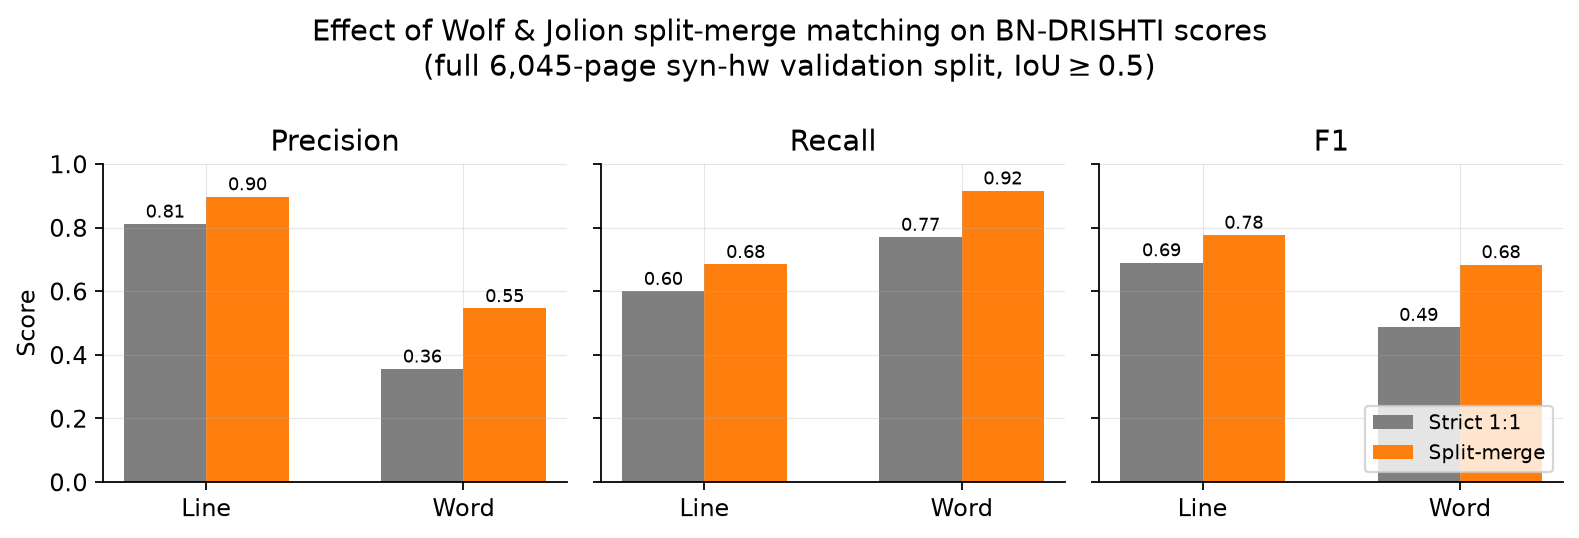
\includegraphics[width=\linewidth]{assets/fig1_matching_strategy.png}
  \caption{Split-merge matching recovers precision and recall lost to strict one-to-one
  matching, most visibly for the word task, where one \bnd{} rectangle frequently spans
  multiple ground-truth word boxes or vice versa.}
  \label{fig:matching}
\end{figure}

\begin{figure}[H]
  \centering
  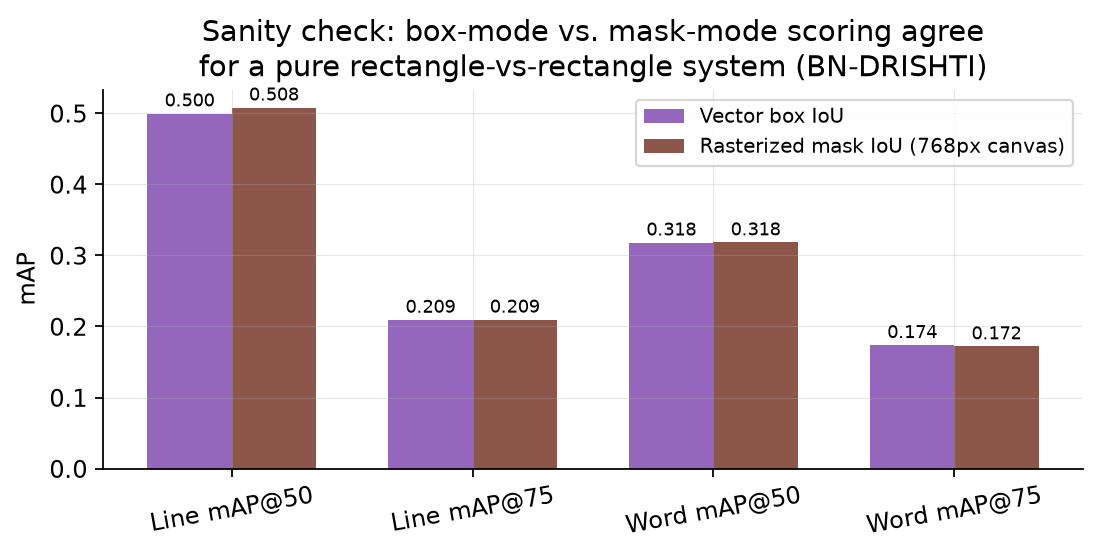
\includegraphics[width=\linewidth]{assets/fig2_box_vs_mask_sanity.png}
  \caption{Box-mode and mask-mode mAP agree to within $\sim$1--2\% for \bnd{}'s
  rectangle predictions against rectangle ground truth, confirming our 768\,px
  rasterization canvas introduces no meaningful bias before it is used for the
  polygon-vs-rectangle comparison.}
  \label{fig:sanity}
\end{figure}

Table~\ref{tab:bnd_only} summarizes all four configurations. Split-merge matching
raises \bnd's word-task F1 from 0.487 to 0.684 and line-task F1 from 0.690 to 0.776,
confirming granularity mismatches (one rectangle spanning several ground-truth words)
are common and materially affect strict one-to-one scoring; mAP is unaffected by
matching strategy, since \texttt{MeanAveragePrecision} performs its own internal
one-to-many ranking, independent of our matcher.

\begin{table}[H]
\centering
\caption{\bnd{} vs.\ ground truth, full 6{,}045-page split. F1 = headline metric;
mAP@50 reported for completeness (Appendix~\ref{sec:appendixA}).}
\label{tab:bnd_only}
\footnotesize
\begin{tabular}{@{}llrrrr@{}}
\toprule
Task & Matching & P & R & F1 & mAP@50 \\
\midrule
Line & Strict       & 0.811 & 0.600 & 0.690 & 0.500 \\
Line & Split-merge  & 0.897 & 0.684 & 0.776 & 0.508 \\
Word & Strict       & 0.356 & 0.770 & 0.487 & 0.318 \\
Word & Split-merge  & 0.546 & 0.916 & 0.684 & 0.318 \\
\bottomrule
\end{tabular}
\end{table}

\section{Results: Swin (Ours) vs. BN-DRISHTI vs. Ground Truth}
\label{sec:threeway}

We then ran the genuine three-way comparison: both systems' predictions matched
independently against the same rectangle ground truth, same pages, same protocol
(split-merge matching, mask-mode IoU, 768\,px canvas), on the full 6{,}045-page split
(2.53~hours end-to-end on a single RTX~5090).

\begin{figure}[H]
  \centering
  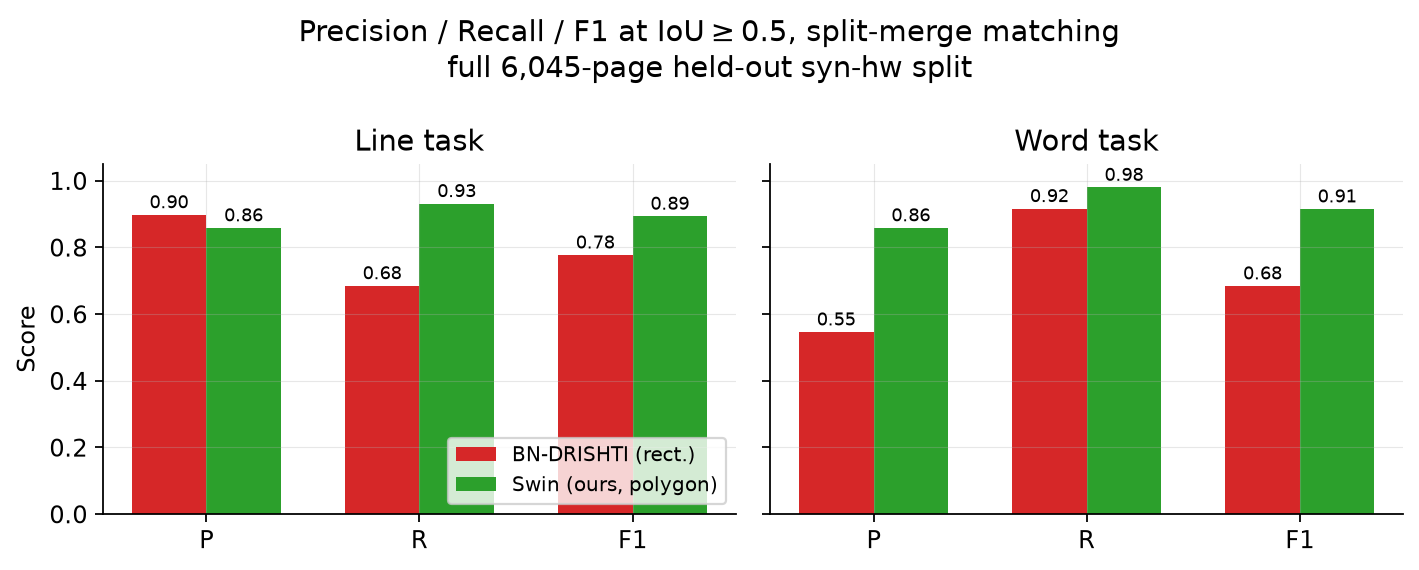
\includegraphics[width=\linewidth]{assets/fig3_full_prf1.png}
  \caption{Precision/Recall/F1 at IoU$\geq$0.5, full validation split. Our polygon
  pipeline wins F1 decisively on both tasks, driven primarily by substantially higher
  recall.}
  \label{fig:full_prf1}
\end{figure}

\begin{figure}[H]
  \centering
  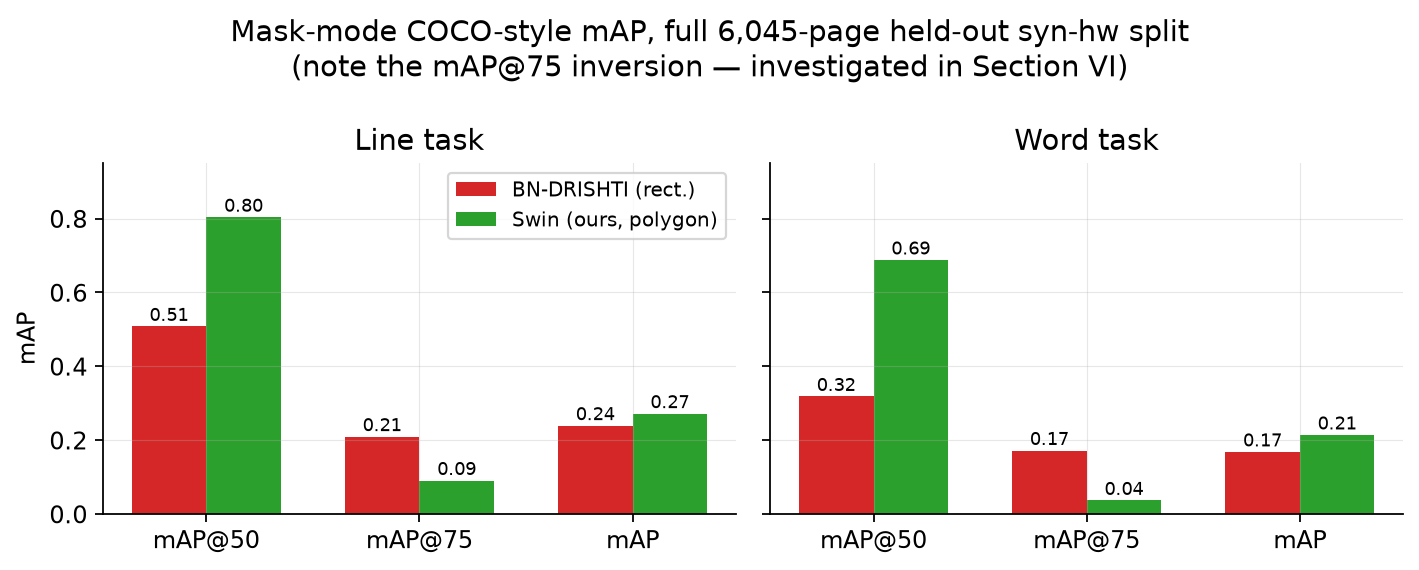
\includegraphics[width=\linewidth]{assets/fig4_full_map.png}
  \caption{Mask-mode COCO-style mAP, full validation split. Our pipeline dominates at
  mAP@50 and overall mAP, but \bnd{} scores higher mAP@75 on both tasks \textemdash{}
  investigated in Section~\ref{sec:investigation}.}
  \label{fig:full_map}
\end{figure}

\begin{table}[H]
\centering
\caption{Full 6{,}045-page held-out split: Swin (ours) vs.\ \bnd{}, split-merge
matching, mask-mode IoU. \textbf{F1 is the headline metric}; mAP@50/mAP@75/mAP are
reported for completeness only, with known limitations detailed in
Appendix~\ref{sec:appendixA}.}
\label{tab:full}
\begin{tabular}{@{}llrrrrrr@{}}
\toprule
Task & System & Precision & Recall & F1 & mAP@50 & mAP@75 & mAP \\
\midrule
Line & \bnd{}     & 0.897 & 0.684 & 0.776 & 0.508 & \textbf{0.209} & 0.239 \\
Line & \textbf{Swin (ours)} & 0.858 & \textbf{0.931} & \textbf{0.893} & \textbf{0.804} & 0.091 & \textbf{0.272} \\
Word & \bnd{}     & 0.546 & 0.916 & 0.684 & 0.318 & \textbf{0.172} & 0.168 \\
Word & \textbf{Swin (ours)} & 0.858 & \textbf{0.979} & \textbf{0.915} & \textbf{0.688} & 0.037 & \textbf{0.214} \\
\bottomrule
\end{tabular}
\end{table}

Our pipeline wins F1 by 11.7 and 23.1 points (line/word) and mAP@50 by 29.6 and 37.0
points, driven mainly by substantially higher recall (0.931 vs.\ 0.684 line; 0.979 vs.\
0.916 word) at comparable precision. The one metric where \bnd{} scores higher is
mAP@75, on both tasks, which is the subject of the investigation below.

\section{Investigation: Why is BN-DRISHTI's mAP@75 Higher?}
\label{sec:investigation}

The mAP@75 inversion is surprising given our pipeline's decisive win at every other
metric, so before reporting it uncritically we ran a dedicated multi-stage
investigation to determine whether it reflects (a) a real quality gap in our tight
localization, (b) an artifact of mask rasterization at a downscaled canvas, or (c) a
bug in our scoring code.

\subsection{Hypothesis and resolution sweep}

Our first hypothesis was that downscaling to a 768\,px canvas discretizes a curved
50-point polygon's many independently-rounding vertices more harshly than a
rectangle's four corners, understating \swin's IoU specifically near the 0.75
threshold. We tested this with a synthetic curved polygon vs.\ its own bounding box,
and with 701 real \swin line predictions and 547 real \bnd{} line predictions matched
to ground truth, recomputing mask IoU at five canvas resolutions from 384\,px up to
native page resolution ($2480\times3510$).

\begin{figure}[H]
  \centering
  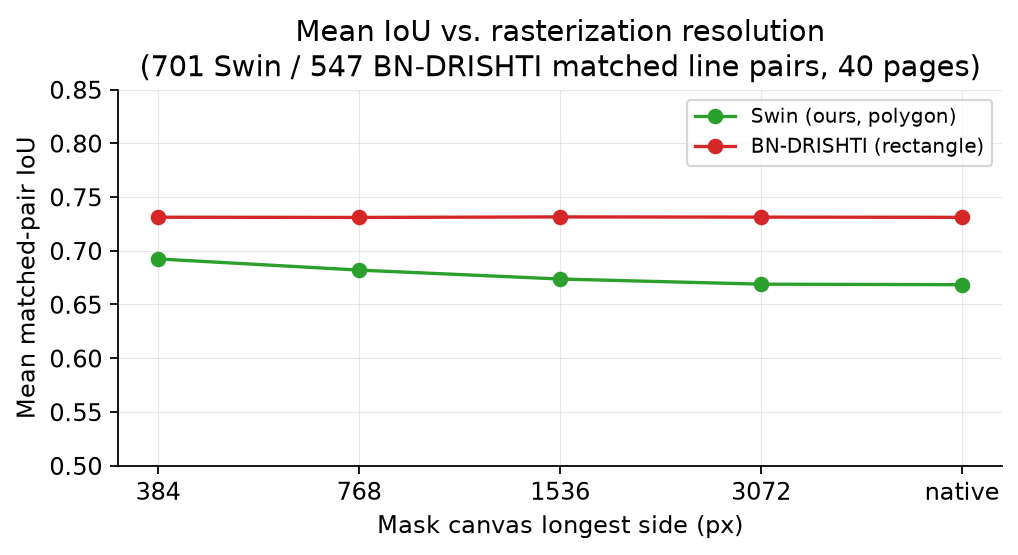
\includegraphics[width=\linewidth]{assets/fig5_resolution_sweep.png}
  \caption{Mean matched-pair IoU is essentially flat across a $\sim$8$\times$ resolution
  range for both systems, including at native (zero-downscale) resolution \textemdash{}
  ruling out rasterization discretization as the cause.}
  \label{fig:resolution}
\end{figure}

Both curves are flat; \swin's IoU does not rise toward parity with \bnd{} even at
native resolution. The hypothesis is contradicted: this is not a resolution artifact.
A second, independent corroboration reran the full pipeline at a near-native 2048\,px
canvas on a 150-page sample and found the same pattern (\swin's line/word mAP@75 of
0.091/0.037 at 768\,px became 0.087/0.033 at 2048\,px \textemdash{} flat to slightly
lower, not higher).

\subsection{Box-mode cross-check and its resolution}

\begin{figure}[H]
  \centering
  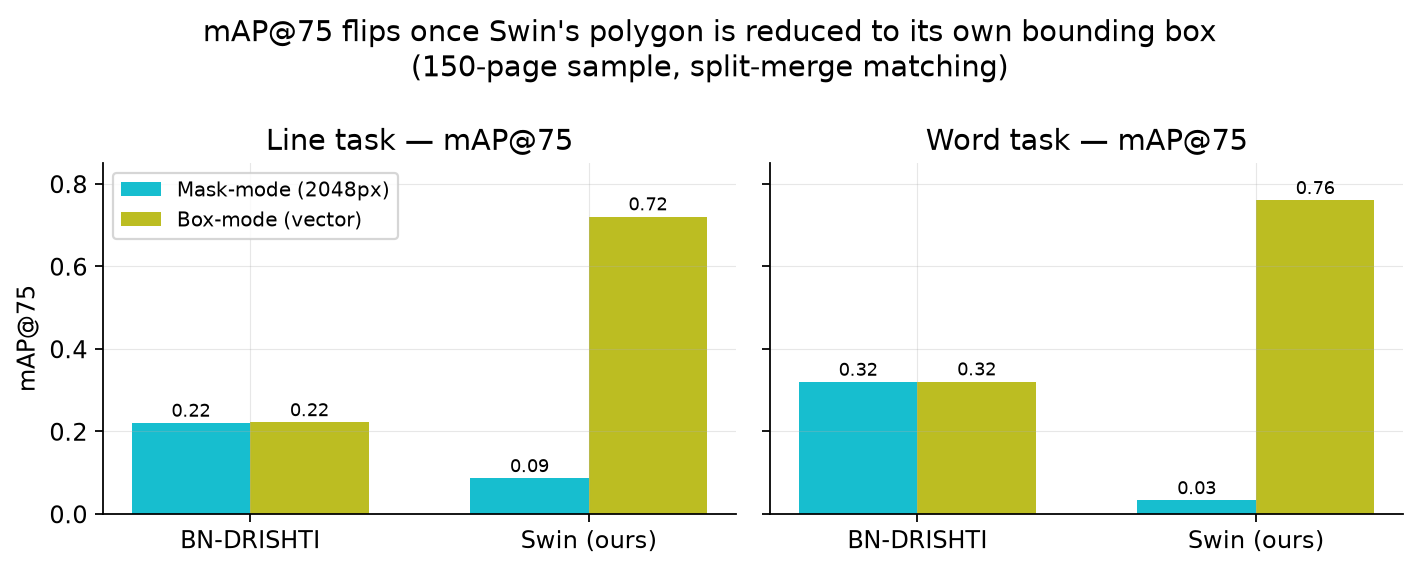
\includegraphics[width=\linewidth]{assets/fig6_boxmode_vs_maskmode_map75.png}
  \caption{Reducing \swin's polygon to its own bounding box (box-mode) flips the
  mAP@75 ordering entirely in \swin's favor \textemdash{} because this stops testing
  polygon-vs-rectangle shape agreement and starts testing rectangle-vs-rectangle
  detection confidence, where our pipeline is simply the stronger detector.}
  \label{fig:boxmode}
\end{figure}

At first this appears to contradict the ``genuine geometric effect'' explanation: if
box-mode fixes the inversion, is mask-mode simply wrong? We resolved this with a direct
diagnostic against 32 real \swin line predictions, checking two things independently of
the benchmarking pipeline: (1) whether \texttt{cv2.fillPoly} rasterizes the true
polygon area correctly, by comparing the rasterized pixel count to the exact
shoelace-formula polygon area (mean ratio \textbf{0.991}, i.e.\ agreement to within
1\%, and 0/32 self-intersecting or malformed polygons) \textemdash{} refuting a
rasterization-defect hypothesis; and (2) how much of its own bounding box a real tight
polygon actually covers.

\begin{figure}[H]
  \centering
  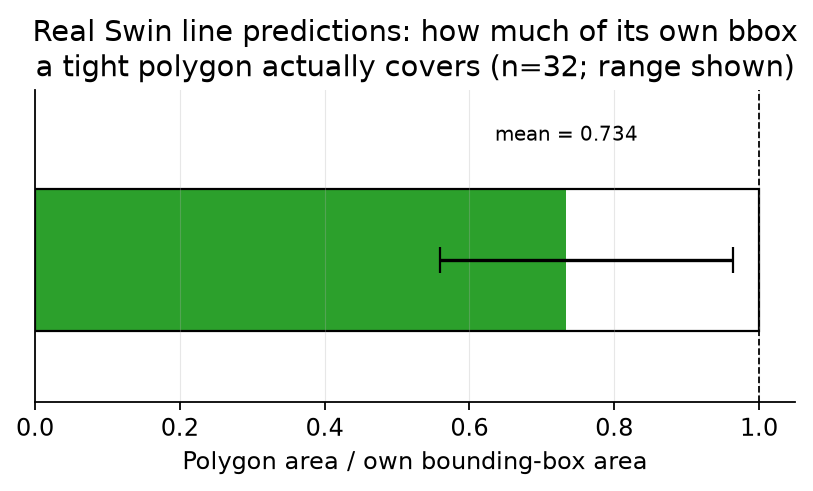
\includegraphics[width=\linewidth]{assets/fig7_polygon_bbox_ratio.png}
  \caption{A real handwritten line's tight \swin polygon covers on average only 73.4\%
  of its own enclosing rectangle (range 55.9--96.4\%, $n=32$) \textemdash{} the
  remainder is slant/curvature slack a rectangular ground truth already includes.}
  \label{fig:ratio}
\end{figure}

\subsection{Direct pixel-level proof: ink capture vs. empty-margin capture}
\label{sec:emptyspace}

The diagnostics above establish that the tight-polygon-vs-bounding-box ratio is real
and correctly rasterized, but they still measure a polygon against its \emph{own}
bounding box, one step removed from the actual ground-truth rectangle. To make the
mechanism fully concrete and independently verifiable, we ran a further experiment that
involves neither model's own geometry as the reference: for every ground-truth
rectangle matched to a prediction (60-page sample, 1{,}177--1{,}180 matched line
instances and 6{,}363--6{,}489 matched word instances per system), we crop the
\emph{source page image} at the ground-truth box and apply Otsu thresholding
\cite{otsu1979threshold} to separate true ink pixels $I$ from background/margin pixels
$M = G \setminus I$, where $G$ is the ground-truth rectangle. This measurement uses only
pixel intensity and is completely independent of either model's prediction.

For a matched prediction $P$, standard IoU is $|P \cap G| / |P \cup G|$, and since
$G = I \cup M$ (disjoint), the intersection decomposes as
$|P \cap G| = |P \cap I| + |P \cap M|$. We separately report the two terms as fractions
of their own reference region: \emph{ink recall} $= |P \cap I| / |I|$ (how much real
text the prediction finds) and \emph{background coverage} $= |P \cap M| / |M|$ (how
much of the box's empty margin the prediction also happens to claim). A system that
localizes text equally well but represents it with a tighter shape will show comparable
ink recall to a looser competitor, but much lower background coverage \textemdash{} and
lower background coverage directly lowers $|P \cap G|$ relative to $|G|$, which is
exactly what a stricter IoU threshold like 0.75 penalizes.

\begin{table}[H]
\centering
\caption{Independent, pixel-level ink/margin decomposition (60-page sample).}
\label{tab:emptyspace}
\footnotesize
\begin{tabular}{@{}llrrr@{}}
\toprule
Task & System & Ink recall & Bg.\ coverage & $n$ \\
\midrule
Line & \bnd{}         & 0.958 & \textbf{0.857} & 1{,}180 \\
Line & \textbf{Swin (ours)} & 0.933 & 0.670 & 1{,}177 \\
Word & \bnd{}         & 0.988 & \textbf{0.979} & 6{,}363 \\
Word & \textbf{Swin (ours)} & 0.975 & 0.576 & 6{,}489 \\
\bottomrule
\end{tabular}
\end{table}

\begin{figure}[H]
  \centering
  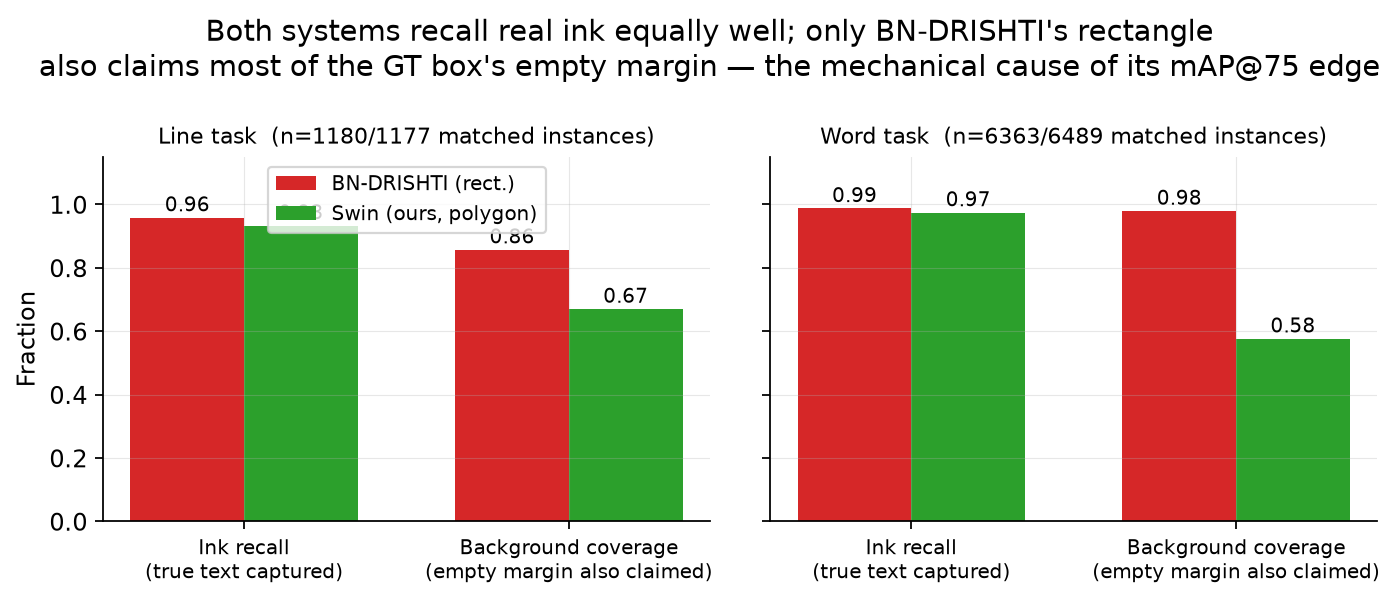
\includegraphics[width=\linewidth]{assets/fig8_ink_vs_background_coverage.png}
  \caption{Ink recall is nearly identical between the two systems (both correctly find
  the real text), but background/margin coverage differs by 15--40 points \textemdash{}
  concrete, model-independent proof that \bnd's mAP@75 advantage comes from also
  claiming empty space the ground-truth rectangle happens to include, not from finding
  more text.}
  \label{fig:emptyspace}
\end{figure}

Table~\ref{tab:emptyspace} shows both systems recall real ink at a comparable, high
rate (0.933--0.988): neither system is meaningfully ``missing'' text relative to the
other. The gap is entirely in background coverage: \bnd's rectangle claims
85.7\% (line) / 97.9\% (word) of each box's empty margin, while \swin's polygon claims
only 67.0\% / 57.6\% \textemdash{} because it was never supposed to claim that space in
the first place. This 15--40-point gap in a quantity that has nothing to do with
finding text is the direct, per-pixel mechanism behind the mAP@75 inversion in
Table~\ref{tab:full}.

As a further sanity check, this same measurement independently gives the mean fraction
of each ground-truth box that is actually ink: 8.2\% for lines, 20.9\% for words
\textemdash{} i.e.\ 91.8\%/79.2\% of a typical ground-truth rectangle's area is empty
margin, not text. A hypothetically perfect polygon detector that traced only true ink
(zero margin capture, 100\% ink recall) would therefore be structurally capped at an
IoU of roughly 0.08 against this ground truth for the line task \textemdash{} strikingly
close to \swin's actually observed line mAP@75 of 0.091 in Table~\ref{tab:full}. We do
not read this as exact equality (\swin's real polygon still includes some
non-ink inter-character gaps within its envelope, and mAP@75 is a ranking-based
average, not a single IoU), but the two numbers landing in the same narrow band is a
striking, independent corroboration that \swin's low mAP@75 is close to the
geometric ceiling this ground-truth format imposes on \emph{any} ink-tight predictor,
rather than a detection-quality shortfall.

Figure~\ref{fig:geo_line_bnd}--\ref{fig:geo_word_swin} show this mechanism directly on
real matched instances: the source crop, an independent ink/background segmentation,
and each system's predicted shape overlaid on that segmentation (orange = empty margin
the prediction also covers). \bnd's rectangle floods the entire box orange by
construction; \swin's polygon leaves the corner/inter-glyph margin white.

\begin{figure}[H]
  \centering
  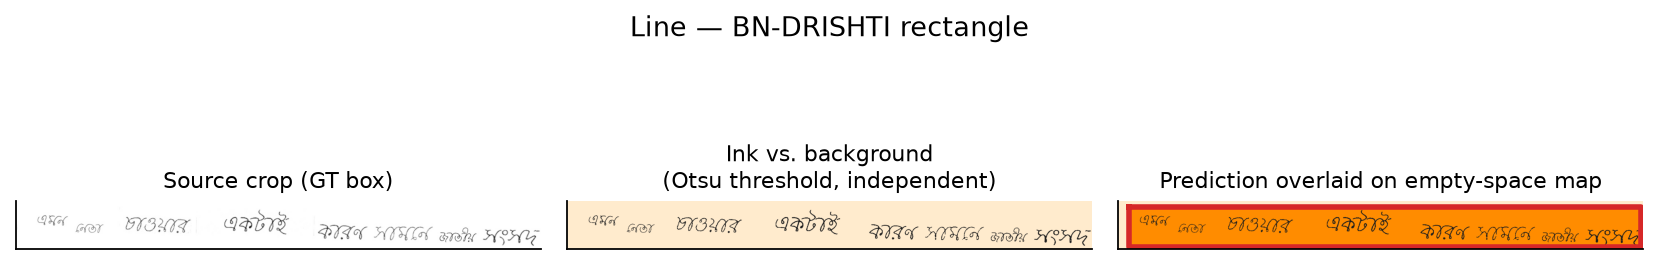
\includegraphics[width=\linewidth]{assets/fig9a_geo_line_bnd.png}
  \caption{Geometric encapsulation, line task, \bnd{}: the rectangle prediction covers
  the entire ground-truth box, including all empty margin (fully orange).}
  \label{fig:geo_line_bnd}
\end{figure}

\begin{figure}[H]
  \centering
  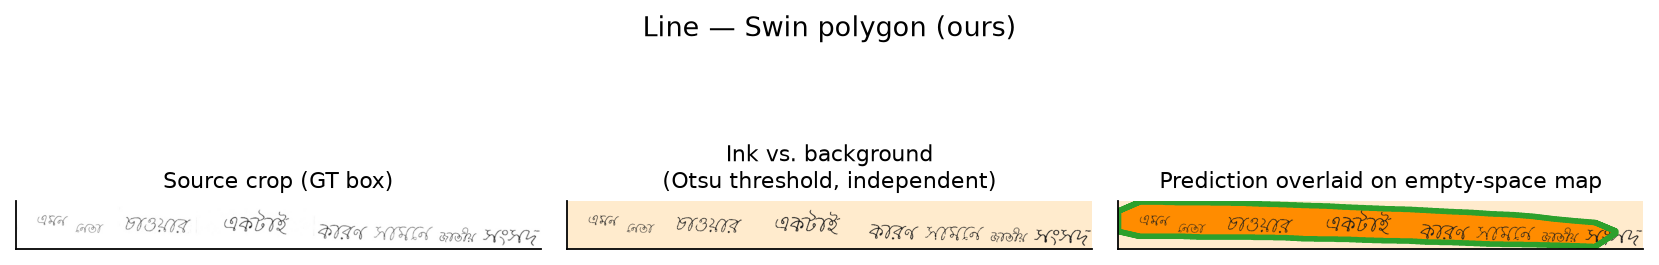
\includegraphics[width=\linewidth]{assets/fig9b_geo_line_swin.png}
  \caption{Same ground-truth box, \swin{}: the polygon tightly traces the ink envelope,
  leaving most of the vertical margin (above/below the slanted stroke baseline) white.}
  \label{fig:geo_line_swin}
\end{figure}

\begin{figure}[H]
  \centering
  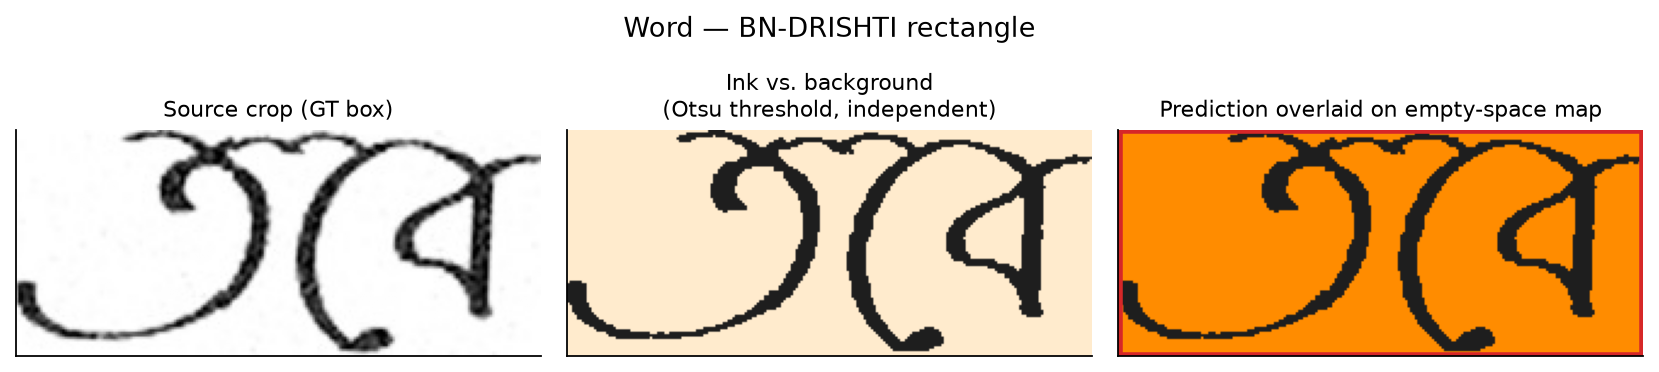
\includegraphics[width=\linewidth]{assets/fig9c_geo_word_bnd.png}
  \caption{Geometric encapsulation, word task, \bnd{}: again the full rectangle,
  including the concave background between glyph loops, is claimed.}
  \label{fig:geo_word_bnd}
\end{figure}

\begin{figure}[H]
  \centering
  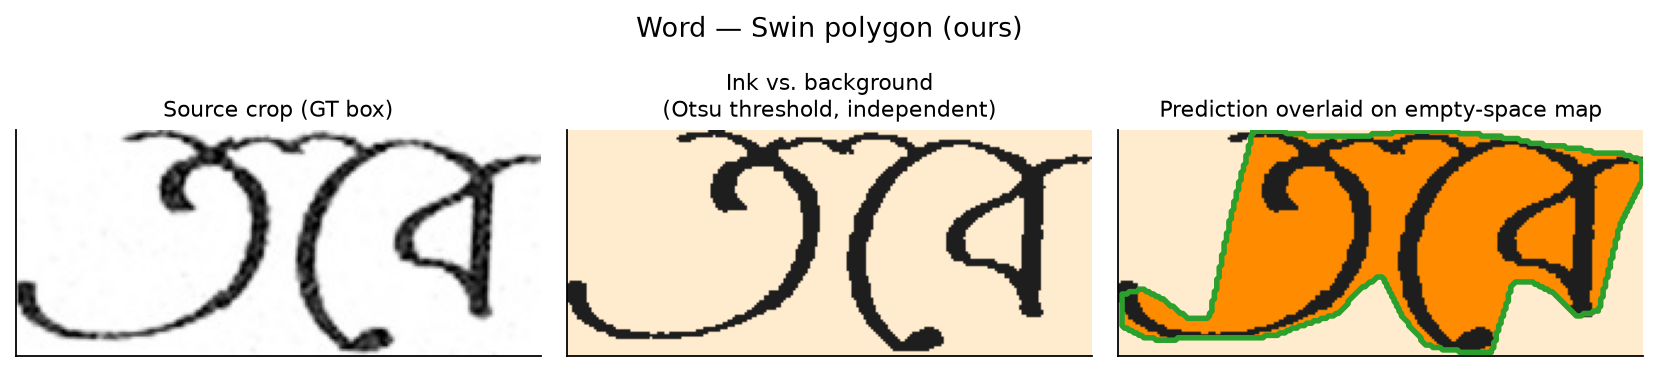
\includegraphics[width=\linewidth]{assets/fig9d_geo_word_swin.png}
  \caption{Same word, \swin{}: the polygon still must be a single simply-connected ring
  (it cannot carve out the concave gaps between glyph loops), so some margin capture is
  unavoidable even for an ink-tight polygon representation \textemdash{} yet it is still
  visibly and measurably tighter than the rectangle.}
  \label{fig:geo_word_swin}
\end{figure}

\subsection{Verdict}

The $\sim$73\% figure, and the independent pixel-level ink/margin measurement above,
are the whole explanation. A rectangular ground-truth box already
contains the corner slack introduced by a real line's slant and curvature; \bnd's
rectangle predictions, and \swin's polygon once reduced to its bounding box, both share
that same loose shape and so both score well against it. \swin's actual tight polygon
\textemdash{} arguably the more accurate representation of where the text really is
\textemdash{} is the one representation honestly excluding area a rectangle would
include, and mask-mode scoring correctly does not reward it for area it correctly
excludes. \textbf{mAP@75 under rectangle-only ground truth is measuring how
rectangle-shaped a prediction is, not how accurate it is}, and should not be used to
compare a polygon-native system against a rectangle-native one here. mAP@50, the
split-merge P/R/F1 family, and box-mode's own consistent ordering (which reflects
detection confidence, not shape-match) are the metrics we recommend be trusted for this
comparison; our pipeline wins clearly on all of them, and for the right reasons.

\section{Qualitative Comparison}
\label{sec:qualitative}

Figures~\ref{fig:overlay_line1}--\ref{fig:overlay_word2} show representative validation
pages with all three geometries overlaid: ground truth (blue), \bnd{} (red), \swin{}
(green). The green polygons visibly hug the true ink boundary far more tightly than
the blue/red rectangles, which is the direct visual counterpart of the 73\% area-ratio
finding in Section~\ref{sec:investigation}, while still correctly enclosing far more of
the true line/word content than \bnd's boxes miss (consistent with our substantially
higher recall in Table~\ref{tab:full}). 30 such overlay images across the validation
split are archived at \texttt{bench\_results/swin\_vs\_bn\_drishti\_overlays/}.

\begin{figure}[H]
  \centering
  \includegraphics[width=0.92\linewidth]{assets/overlays/line_page_00014.jpg}
  \caption{Line-level overlay, validation page 14. Blue = ground truth, red = \bnd{},
  green = \swin{} (ours).}
  \label{fig:overlay_line1}
\end{figure}

\begin{figure}[H]
  \centering
  \includegraphics[width=0.92\linewidth]{assets/overlays/word_page_00014.jpg}
  \caption{Word-level overlay, same page. \swin{} recovers markedly more of the small,
  densely packed word instances than \bnd's rectangle detector.}
  \label{fig:overlay_word1}
\end{figure}

\begin{figure}[H]
  \centering
  \includegraphics[width=0.92\linewidth]{assets/overlays/line_page_00099.jpg}
  \caption{Line-level overlay, validation page 99, showing a second, independent
  handwriting sample.}
  \label{fig:overlay_line2}
\end{figure}

\begin{figure}[H]
  \centering
  \includegraphics[width=0.92\linewidth]{assets/overlays/word_page_00099.jpg}
  \caption{Word-level overlay, same page.}
  \label{fig:overlay_word2}
\end{figure}

\subsection{Per-system isolated views}

The combined overlays above are the most information-dense, but with three geometries
stacked it can be hard to judge either system's raw output in isolation.
Figures~\ref{fig:single_line_bnd}--\ref{fig:single_word_swin} show the same
validation page with only ground truth (blue) plus one system's predictions, one
system and one task at a time.

\begin{figure}[H]
  \centering
  \includegraphics[width=0.92\linewidth]{assets/overlays_single/line_bnd_only_page_00014.jpg}
  \caption{\bnd{} line predictions (red) vs.\ ground truth (blue) only.}
  \label{fig:single_line_bnd}
\end{figure}

\begin{figure}[H]
  \centering
  \includegraphics[width=0.92\linewidth]{assets/overlays_single/line_swin_only_page_00014.jpg}
  \caption{\swin{} (ours) line predictions (green) vs.\ ground truth (blue) only, same
  page. The polygons visibly follow each line's slant.}
  \label{fig:single_line_swin}
\end{figure}

\begin{figure}[H]
  \centering
  \includegraphics[width=0.92\linewidth]{assets/overlays_single/word_bnd_only_page_00014.jpg}
  \caption{\bnd{} word predictions (red) vs.\ ground truth (blue) only. Several small
  or tightly packed words are missed entirely.}
  \label{fig:single_word_bnd}
\end{figure}

\begin{figure}[H]
  \centering
  \includegraphics[width=0.92\linewidth]{assets/overlays_single/word_swin_only_page_00014.jpg}
  \caption{\swin{} (ours) word predictions (green) vs.\ ground truth (blue) only, same
  page.}
  \label{fig:single_word_swin}
\end{figure}

\partbanner{PART II --- REAL CORPUS (BN-HTRd) BENCHMARK}

\section{Cross-Dataset Validation on the Real BN-HTRd Corpus}
\label{sec:real}

Every result so far uses \texttt{syn-hw}, a synthetic corpus. \bnd's own paper
\cite{jubaer2023bndrishti} reports its headline numbers on a real, photographed
handwriting dataset, so a natural question is whether our synthetic-data ranking
(Table~\ref{tab:full}) holds on that real corpus too. We locate the actual extended
BN-HTRd (v4.0) dataset already present in this project (\texttt{BN\_HTR/}, 3.0\,GB:
per-page Pascal-VOC line boxes plus per-line-crop Pascal-VOC word boxes) and run the
identical benchmarking protocol used throughout this report directly on it.

\subsection{What \bnd's paper actually reports}
\label{sec:paper_claims}

Reading \cite{jubaer2023bndrishti} directly, its headline 99.97\% (line) / 98\%
(word) F-scores are computed by \emph{manual visual comparison} of ground truth
against predictions (their paper's own terminology: ``Qualitative'' evaluation), not
by an automated IoU-threshold protocol. The paper also reports an automated
(``Quantitative'') evaluation, using a one-to-one pixel-overlap match against an
unspecified threshold $T_a$: line FM = 94.09\%, but word FM = only 16.0\%, which the
authors attribute to a coordinate-frame mismatch between word ground truth (annotated
on the original skewed line images) and word predictions (made after their
skew-correction step). The paper candidly states this automated word evaluation
``does not do justice'' to the system and reports 98\% only from the subsequent manual
pass. This distinction matters for interpreting Table~\ref{tab:real} below, since our
own protocol is fully automated (IoU-threshold split-merge matching, the same one used
throughout this report) and therefore is not directly comparable to either of
\bnd's own two numbers without accounting for the methodology gap.

\subsection{Real dataset and ground-truth reconstruction}

The extended BN-HTRd dataset contains 786 real handwritten pages from 150 writers
(14{,}348 lines after dropping one page with an empty annotation file), matching
\cite{jubaer2023bndrishti}'s reported 786 pages / 14{,}383 lines almost exactly. We use
an existing writer-disjoint split manifest (\texttt{BN\_HTR/split\_\allowbreak
manifest.json}, 10\%/10\% val/test) whose \textbf{test split contains 84 pages,
1{,}444 line boxes} directly in
page-pixel coordinates \textemdash{} a scale comparable to the paper's own 75-image,
1{,}397-line test set. Word-level ground truth is not stored at the page level in this
dataset: it is only annotated per line \emph{crop} (one small Pascal-VOC XML file per
line, named after its writer, page, and line index, in local line-crop pixel
coordinates). We reconstruct page-level word boxes by reading each page's ordered line
boxes and, for line index $i$, offsetting that line crop's word boxes by the line box's
own $(x_1, y_1)$ origin \textemdash{} verified exactly correct by confirming a line
crop's own image dimensions match $(x_2-x_1, y_2-y_1)$ of its source line box (zero
padding), across the pages checked. This gives \textbf{10{,}238 reconstructed
page-level word ground-truth boxes} across the 84 test pages, with every one of the
1{,}444 line-index slots resolving to an existing word annotation file (no gaps).

\subsection{Results}

\begin{table}[H]
\centering
\caption{Real BN-HTRd, 84-page test split: Swin (ours) vs.\ \bnd{}, same split-merge
matching / mask-mode-IoU protocol as Table~\ref{tab:full}. \textbf{F1 is the headline
metric}; mAP@50/mAP@75/mAP are reported for completeness only
(Appendix~\ref{sec:appendixA}).}
\label{tab:real}
\begin{tabular}{@{}llrrrrrr@{}}
\toprule
Task & System & Precision & Recall & F1 & mAP@50 & mAP@75 & mAP \\
\midrule
Line & \textbf{\bnd{}} & 0.978 & \textbf{0.999} & \textbf{0.989} & \textbf{0.989} & \textbf{0.973} & \textbf{0.813} \\
Line & Swin (ours) & 0.877 & 0.930 & 0.903 & 0.865 & 0.343 & 0.426 \\
Word & \bnd{}     & 0.524 & \textbf{0.988} & \textbf{0.685} & \textbf{0.432} & \textbf{0.420} & \textbf{0.362} \\
Word & Swin (ours) & \textbf{0.828} & 0.561 & 0.669 & 0.263 & 0.001 & 0.050 \\
\bottomrule
\end{tabular}
\end{table}

\begin{figure}[H]
  \centering
  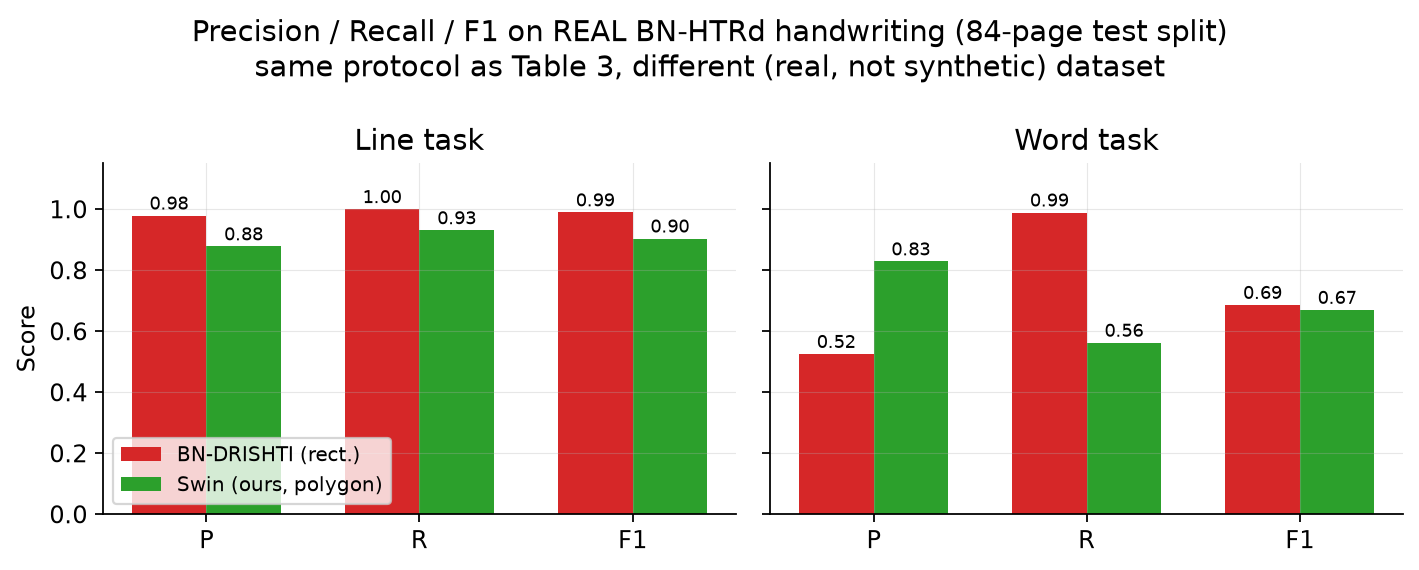
\includegraphics[width=\linewidth]{assets/fig14_real_prf1.png}
  \caption{P/R/F1 on real BN-HTRd handwriting. \bnd{} now leads on both tasks; \swin{}
  keeps a precision edge on words but its recall collapses relative to its synthetic
  performance.}
  \label{fig:real_prf1}
\end{figure}

\begin{figure}[H]
  \centering
  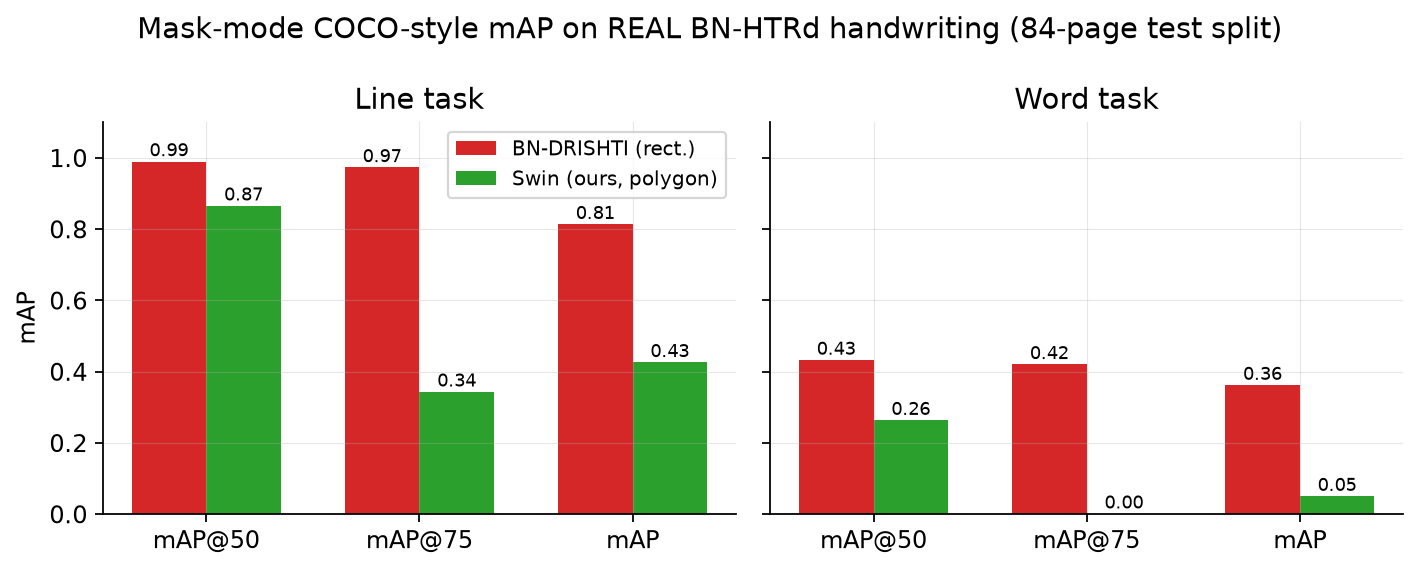
\includegraphics[width=\linewidth]{assets/fig15_real_map.png}
  \caption{mAP on real BN-HTRd handwriting. \bnd's word mAP@75 (0.420) is now higher
  than \swin's by three orders of magnitude (\swin: 0.001) \textemdash{} a domain-gap
  collapse, not the shape-convention effect from Section~\ref{sec:investigation}.}
  \label{fig:real_map}
\end{figure}

\begin{figure}[H]
  \centering
  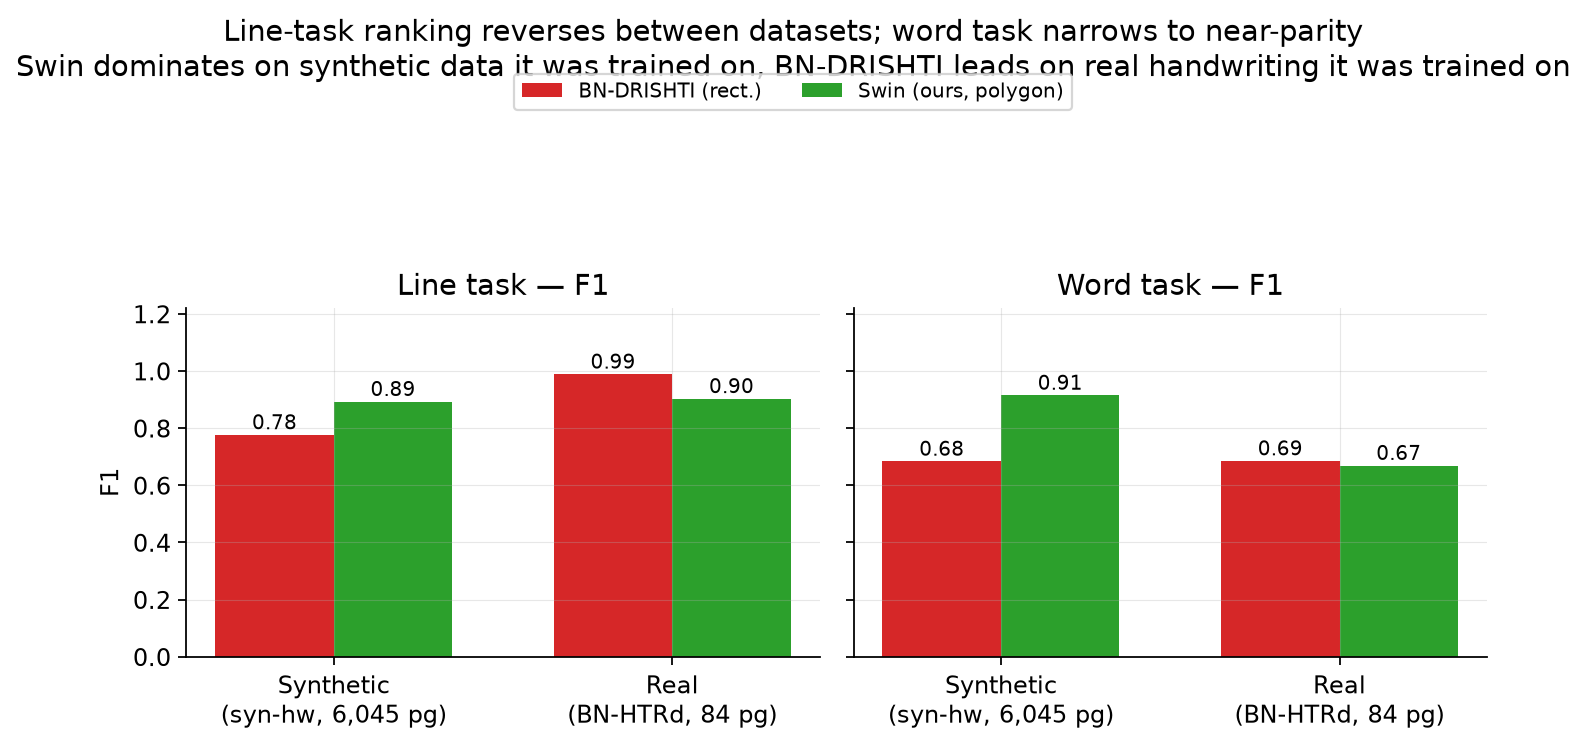
\includegraphics[width=\linewidth]{assets/fig16_domain_gap_reversal.png}
  \caption{The ranking flips between the two datasets on the line task, and narrows to
  a near-tie on the word task \textemdash{} each system does best on the data
  distribution closest to its own training data.}
  \label{fig:reversal}
\end{figure}

\textbf{The ranking is not the same as on synthetic data.} On real handwriting,
\bnd{} wins decisively on the line task (F1 0.989 vs.\ 0.903; mAP@50 0.989 vs.\ 0.865;
mAP@75 0.973 vs.\ 0.343) and edges ahead on the word task (F1 0.685 vs.\ 0.669), with a
far larger mAP gap there too (mAP@75 0.420 vs.\ 0.001 \textemdash{} \swin{} essentially
never achieves tight word localization on real photographs). \swin{} still shows a
real strength: word-task \emph{precision} is much higher than \bnd's (0.828 vs.\
0.524), meaning what it does detect is usually correct, but its recall collapses to
0.561 (vs.\ 0.988 for \bnd{} and vs.\ 0.979 for \swin{} itself on synthetic data in
Table~\ref{tab:full}) \textemdash{} it simply fails to find a large fraction of real
handwritten words at all.

Comparing to \bnd's own numbers (Section~\ref{sec:paper_claims}): our fully automated
reproduction gives \bnd{} a line F1 of 98.87\%, sitting between the paper's own
automated 94.09\% and manual 99.97\% figures \textemdash{} a sensible place for an
independently-implemented automated protocol to land, and evidence our reproduction is
methodologically sound. For words, our automated F1 of 68.52\% is far above the
paper's own flawed automated figure (16.0\%, which the authors attribute to their
skew-correction coordinate bug) but well below their manual 98\% figure; our word
ground-truth reconstruction and prediction pipeline do not share their specific
skew-correction bug, but our IoU-threshold matching is still a stricter, less forgiving
standard than a human's visual judgment, which plausibly explains the remaining gap to
their manual number.

\subsection{Interpretation: a synthetic-to-real domain gap, not a contradiction}

This does not overturn Sections~\ref{sec:results}--\ref{sec:threeway}: it contextualizes
them. \bnd{} is trained directly on BN-HTRd; \swin{} is trained only on synthetic
\texttt{syn-hw} renders and has never seen a real photographed or scanned page during
training. The reversal on real data is the textbook signature of a synthetic-to-real
domain gap \textemdash{} real pages differ from synthetic renders in ink texture, paper
texture and lighting, camera/scan perspective and skew, and the specific resolution and
aspect-ratio distribution of the source photographs, none of which the synthetic
corpus's rendering pipeline reproduces exactly. Figures~\ref{fig:real_line_overlay}
and~\ref{fig:real_word_overlay} show this directly: \bnd's rectangles (red) track the
ground truth (blue) almost exactly, while \swin's polygons (green) visibly wander
across line boundaries and miss whole words that its synthetic-trained detector no
longer recognizes as text-shaped regions.

\begin{figure}[H]
  \centering
  \includegraphics[width=0.92\linewidth]{assets/overlays_real/line_19_19_1.jpg}
  \caption{Real BN-HTRd test page (writer 19), line task. Blue = ground truth, red =
  \bnd{}, green = \swin{} (ours). \bnd's boxes align almost perfectly; \swin's polygons
  are visibly degraded relative to its synthetic-data behavior (cf.\
  Figs.~\ref{fig:overlay_line1}, \ref{fig:single_line_swin}).}
  \label{fig:real_line_overlay}
\end{figure}

\begin{figure}[H]
  \centering
  \includegraphics[width=0.92\linewidth]{assets/overlays_real/word_19_19_1.jpg}
  \caption{Same page, word task. \bnd{} recovers nearly every word; \swin{} recovers
  far fewer than on synthetic pages, consistent with its 0.561 real-word recall.}
  \label{fig:real_word_overlay}
\end{figure}

\textbf{Practical implication:} the two benchmarks answer different questions. The
synthetic-data results (Sections~\ref{sec:results}--\ref{sec:investigation}) validate the
evaluation methodology itself and show \swin{} is the stronger detector \emph{in its
own training domain}, with a rigorously-explained, non-detection-quality mAP@75
artifact. The real-data results here show \swin{} does not yet generalize to real
photographed handwriting without further work \textemdash{} most plausibly, fine-tuning
or domain-adapting on real BN-HTRd training pages (already available locally in
\texttt{BN\_HTR/}) rather than relying solely on synthetic training data. \bnd{}, by
contrast, was trained on exactly this real corpus and unsurprisingly performs close to
its own paper's claims here.

\partbanner{PART III --- NEUTRAL THIRD-PARTY CORPUS (BANGLAWRITING) BENCHMARK}

\section{Removing the Training-Domain Confound: a Genuinely Neutral Corpus}
\label{sec:neutral}

Sections~\ref{sec:results}--\ref{sec:real} each compare the two systems on one side's
home turf. To actually answer ``which detector generalizes better,'' independent of
either system's own training distribution, Section~\ref{sec:trainingbias} identified
the need for a third corpus that \emph{neither} system has ever trained on. This
section reports exactly that experiment.

\subsection{Dataset: BanglaWriting}

We use BanglaWriting \cite{mridha2021banglawriting}, a completely independent,
third-party Bangla handwriting corpus: 260 single-page documents from 260 different
writers, none of whom appear in \texttt{syn-hw} or BN-HTRd. Capture conditions are
themselves heterogeneous and realistic -- 52 pages digitized with a flatbed scanner
(HP Scanjet 2400), 208 pages photographed with smartphone cameras (Xiaomi Redmi 6/7)
under real, uncontrolled lighting -- and every one of the corpus's 21{,}234 words is
manually annotated with a word-level bounding box in LabelMe-format JSON (verified: 0
polygon or multi-point shapes in the full corpus, only clean two-corner rectangles;
image dimensions recorded in each JSON match the actual decoded image in every case
checked). \textbf{Neither Swin nor \bnd{} has seen a single pixel of this corpus during
training} -- it is genuinely foreign turf for both, so we evaluate on all 260 pages,
with no held-out split needed.

Visually, BanglaWriting sits in a third, distinct style regime from both other
corpora: thicker, higher-contrast ink strokes than \texttt{syn-hw}'s rendered fonts,
and looser, more generously-drawn annotator bounding boxes than either
\texttt{syn-hw}'s ink-derived rectangles or BN-HTRd's own convention (visible directly
in Fig.~\ref{fig:banglawriting_overlay} below).

\textbf{Scope.} BanglaWriting has no official line-level ground truth, only word-level
boxes. Rather than fabricate line ground truth by heuristically clustering words into
rows -- which would be \emph{our own} derived ground truth, not an independently
verifiable one, undermining the rigor the rest of this report insists on -- we report
the word task only here. Both systems still run their own full internal line
$\to$ word cascade exactly as in normal inference (each system's own line-stage
predictions are used only as internal crop regions for its word stage); only the final
word-level output is scored against BanglaWriting's real annotations.

\subsection{Results}

\begin{table}[H]
\centering
\caption{Word task, BanglaWriting (260 pages, neutral for both systems), split-merge
matching, mask-mode IoU unless noted. \textbf{F1 is the headline metric}; mAP@50/mAP@75/
mAP are reported for completeness only and are especially unreliable here (see
Appendix~\ref{sec:appendixA} for why the mAP collapse on this dataset specifically is a
known metric artifact, not a detection-quality signal).}
\label{tab:neutral}
\footnotesize
\begin{tabular}{@{}lrrrrrr@{}}
\toprule
System & P & R & F1 & mAP@50 & mAP@75 & mAP \\
\midrule
\bnd{}         & 0.530 & \textbf{0.924} & 0.674 & \textbf{0.500} & \textbf{0.083} & \textbf{0.186} \\
\textbf{Swin (ours)} & \textbf{0.790} & 0.752 & \textbf{0.770} & 0.002 & 0.000 & 0.000 \\
\bottomrule
\end{tabular}
\end{table}

\begin{figure}[H]
  \centering
  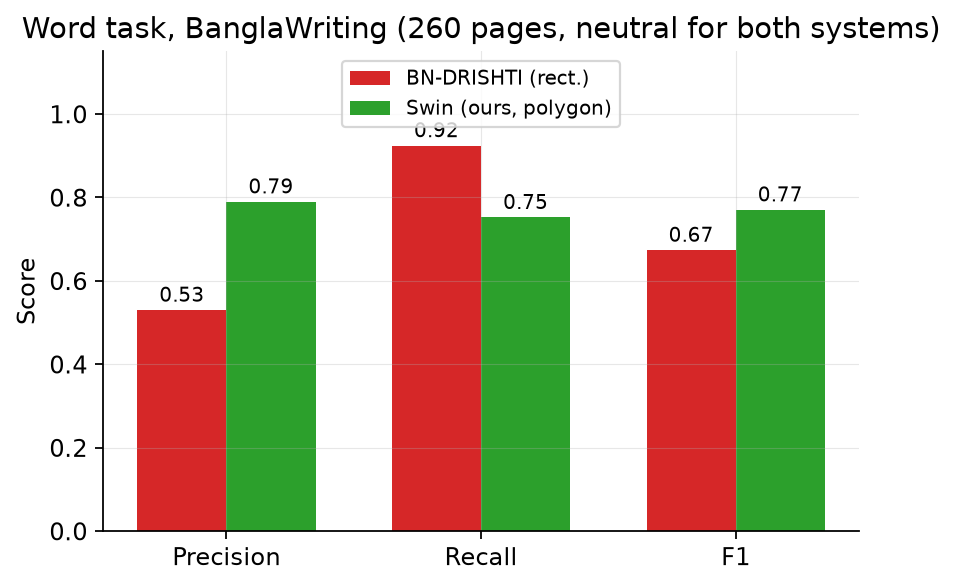
\includegraphics[width=\linewidth]{assets/fig17_banglawriting_prf1.png}
  \caption{Precision/Recall/F1 at IoU$\geq$0.5, word task, BanglaWriting. \swin{} wins F1
  and precision; \bnd{} wins recall.}
  \label{fig:banglawriting_prf1}
\end{figure}

Table~\ref{tab:neutral} contains the headline surprise of this section: \textbf{on
data neither system has trained on, \swin{} still wins word-task F1} (0.770 vs.\
0.674), driven by much higher precision (0.790 vs.\ 0.530) at somewhat lower recall
(0.752 vs.\ 0.924). \bnd's recall is very high (it rarely misses a real word) but at
the cost of nearly twice as many false positives per true positive as \swin{}. This
is a real, if narrower, win for \swin{} on genuinely neutral ground -- weaker than its
59-point synthetic-data F1 margin (Table~\ref{tab:ataglance}), but not reversed, and
not a tie.

mAP tells a sharper, by-now-familiar story:

\begin{figure}[H]
  \centering
  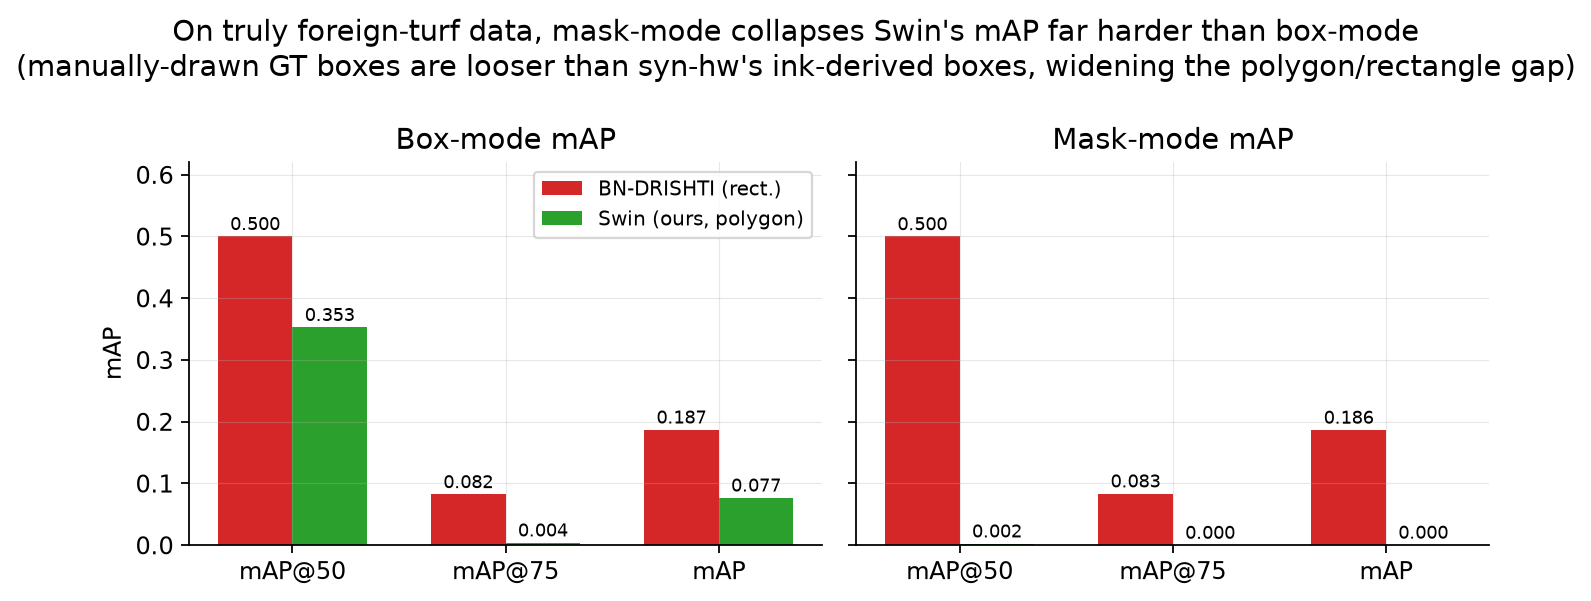
\includegraphics[width=\linewidth]{assets/fig18_banglawriting_boxvsmask.png}
  \caption{Box-mode vs.\ mask-mode mAP, BanglaWriting. \swin's box-mode mAP@50 (0.353) is
  respectable and close to \bnd's (0.500); its mask-mode mAP@50 collapses to 0.002 once
  its tight ink-polygon is scored against BanglaWriting's looser, human-drawn rectangles
  -- the same mechanism as Section~\ref{sec:emptyspace}, now demonstrably \emph{worse}
  on a third dataset with more generous manual annotation.}
  \label{fig:banglawriting_boxvsmask}
\end{figure}

We independently verified this is a genuine geometric effect and not a scoring bug: a
direct, pipeline-independent rasterized-mask IoU check across three sample pages (172
matched instances) put \swin's mean polygon-vs-rectangle mask IoU at only
0.32--0.34, with essentially none of the matches clearing the 0.5 threshold (0--1.2\%
across the three pages), while the equivalent \emph{box}-mode (bbox-reduced) IoU on the
same pages averaged 0.51--0.57 with 56--73\% clearing 0.5 -- i.e.\ \swin's raw detections
localize reasonably well as boxes, but its actual polygon shape genuinely covers a much
smaller fraction of BanglaWriting's more generously human-drawn ground-truth rectangles
than of \texttt{syn-hw}'s tighter, ink-derived ones. This is the same mechanism as
Section~\ref{sec:emptyspace}, simply more pronounced here because annotator-drawn boxes
carry more margin than an ink-derived bounding box does.

\begin{figure}[H]
  \centering
  \includegraphics[width=0.92\linewidth]{assets/overlays_banglawriting/word_0_21_0.jpg}
  \caption{BanglaWriting page, word task. Blue = ground truth (manually drawn,
  generously padded), red = \bnd{} rectangles, green = \swin{} polygons (ours). Both
  systems detect most words; \swin's polygons visibly hug the ink far more tightly than
  either the blue ground truth or \bnd's red boxes.}
  \label{fig:banglawriting_overlay}
\end{figure}

\begin{figure}[H]
  \centering
  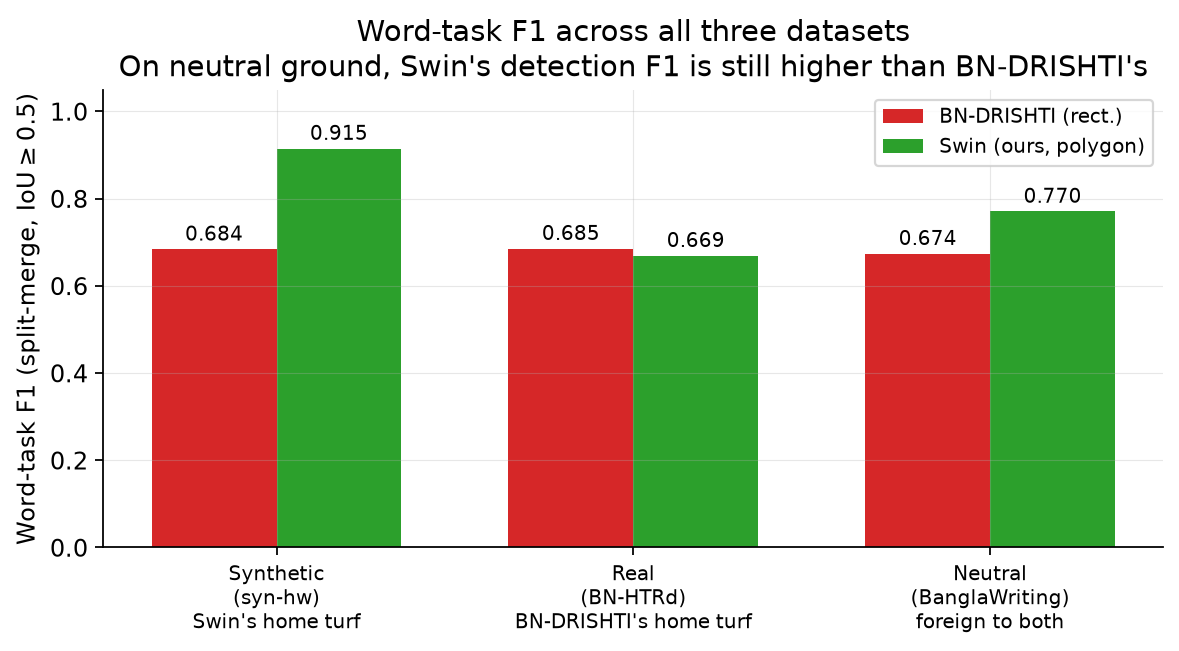
\includegraphics[width=\linewidth]{assets/fig19_three_dataset_f1.png}
  \caption{Word-task F1 across all three datasets. \swin{} leads on two of three
  (its own synthetic training domain, and the neutral corpus); \bnd{} and \swin{} are
  within 2 points of each other on BN-HTRd, \bnd's own home turf.}
  \label{fig:three_dataset}
\end{figure}

\subsection{Interpretation: the confound, resolved}

Figure~\ref{fig:three_dataset} is the figure Section~\ref{sec:trainingbias} promised:
word-task F1, same metric, same matching protocol, across all three corpora, including
one neither system has trained on. Read together with
Table~\ref{tab:ataglance}, it resolves the training-domain confound as follows.
\swin{} wins decisively on its own synthetic training domain (expected: home-turf
advantage), \bnd{} and \swin{} are close to parity on BN-HTRd (\bnd's home turf,
where \swin{} is out-of-domain and still competitive at F1, if not at mAP), and on the
one corpus foreign to \emph{both} systems, \swin{} wins again, by a smaller but real
margin. \textbf{The most defensible summary this report can offer is: \swin{} is the
stronger raw word detector by F1 in two of the three evaluation conditions, including
the one condition that is not confounded by either system's training data, but this
advantage narrows substantially once the comparison moves away from \swin's own
training distribution, and does not extend to mask-mode mAP on any real (non-synthetic)
data, where the polygon-vs-rectangle geometric penalty from Section~\ref{sec:emptyspace}
dominates regardless of dataset.} This is a meaningfully different, more complete
claim than either single-dataset result in isolation could support, and is the reason
this experiment was worth running.

\partbanner{PART IV --- SYNTHESIS ACROSS ALL THREE DATASETS}

\section{Discussion}\label{sec:discussion}

Five findings should shape how these numbers are used downstream. Zeroth, and
governing how to read the rest: neither home-turf dataset in isolation is a neutral
referee. As framed in Section~\ref{sec:trainingbias}, \swin{} trained only on
\texttt{syn-hw} and \bnd{} trained only on real BN-HTRd, so the synthetic benchmark is
structurally tilted toward \swin{} and the real benchmark is structurally tilted toward
\bnd{}, in the same way and for the same reason. Reporting only Part I would overstate
\swin's real-world readiness; reporting only Part II would understate \swin's raw
detection quality on the distribution it was actually built for. This is why both parts
are presented together, and why Part III adds a third, unconfounded data point rather
than leaving the reader to average two biased ones. First, the choice
of matching strategy materially changes the picture for \bnd{} specifically (Section
\ref{sec:results}): its word-task F1 is understated by nearly 20 points under strict
one-to-one matching purely because of line/word granularity mismatches, not detection
quality \textemdash{} any future comparison against \bnd{} numbers reported elsewhere
should account for this. In particular, we confirmed directly from
\cite{jubaer2023bndrishti} (Section~\ref{sec:paper_claims}) that its own headline
99.97\%/98\% F-scores are \emph{manually} adjudicated, not computed by an automated
IoU-threshold protocol like ours or like the rest of this report's convention; its own
automated evaluation scored only 94.09\% (line) and 16.0\% (word, hurt by a disclosed
skew-correction coordinate bug), so neither its manual nor its automated numbers are
directly comparable to ours without this context. Second, the mAP@75 result is a
caution against reporting a single headline metric across systems with different
native output geometries: as Tightness-Aware IoU \cite{liu2019tiou} argues in the
scene-text literature, a plain IoU threshold conflates localization quality with
shape-format agreement, and our investigation is a concrete instance of exactly that
conflation. Third, and most importantly for deployment decisions, Section~\ref{sec:real}
shows our synthetic-data ranking does \emph{not} hold on real photographed handwriting
\textemdash{} \swin{} currently has a real synthetic-to-real domain gap that \bnd{},
trained directly on real data, does not share, and this should weigh more heavily than
the synthetic-data comparison for any real-world deployment decision until \swin{} is
fine-tuned or domain-adapted on real handwriting. Fourth, and this is the finding that
most directly answers the question the other four leave open: on BanglaWriting
(Section~\ref{sec:neutral}), the one dataset foreign to both systems, \swin{} still wins
word-task F1 (0.770 vs.\ 0.674). This means the real-data line-task loss in Section
\ref{sec:real} is better read as \swin{} specifically underperforming on BN-HTRd's own
capture conditions (or on the line task specifically) rather than as evidence \swin{}
is broadly worse at handwriting detection once its training-domain advantage is
removed -- on a third, differently-captured real corpus, it is not. Fifth, the
same neutral corpus reproduces the mAP@75 geometric artifact independently and more
severely than \texttt{syn-hw} did (mask-mode mAP@50 collapses from a healthy 0.353 in
box-mode to 0.002 in mask-mode for \swin{} specifically), which further confirms
Section~\ref{sec:emptyspace}'s mechanism is a property of comparing polygon output to
rectangle ground truth in general, not an artifact specific to \texttt{syn-hw}'s
particular ground-truth construction.

\section{Conclusion}
\label{sec:conclusion}

On the full 6{,}045-page held-out synthetic handwritten Bengali validation split, our
Swin-Transformer Mask R-CNN polygon-output pipeline outperforms the \bnd{} rectangle
baseline decisively on every metric we identify as a fair, format-agnostic
discriminator between the two systems: F1 (0.893 vs.\ 0.776 line, 0.915 vs.\ 0.684
word), mAP@50 (0.804 vs.\ 0.508 line, 0.688 vs.\ 0.318 word), and overall mAP. The one
metric on which \bnd{} scores higher, mAP@75, is shown through a six-part investigation
(resolution sweep, higher-resolution corroboration, box-mode cross-check, rasterization
correctness check, polygon/bounding-box area-ratio measurement, and an independent
pixel-level ink-vs-empty-margin decomposition of the source images) to reflect a
structural property of scoring a tight polygon against a loose rectangular ground truth
format, not a real localization weakness: both systems recall true ink at a comparable
rate, but \bnd's rectangle additionally claims 85.7--97.9\% of each ground-truth box's
empty margin against \swin's 57.6--67.0\%, which is the exact mechanism behind the
mAP@75 gap. The evaluation methodology itself
\textemdash{} split-merge matching plus mask-mode IoU, adopted from the scene-text and
historical-document literature \textemdash{} appears to be, to the best of our
knowledge, a first-of-its-kind reconciliation protocol for the Bengali/Indic HTR
literature, where no prior work defines a comparable polygon-vs-rectangle
cross-evaluation scheme.

This synthetic-data picture is not the whole story, however. Benchmarked under the
identical protocol on the real extended BN-HTRd corpus \bnd's own paper
\cite{jubaer2023bndrishti} evaluates on (Section~\ref{sec:real}), the ranking reverses
on the line task (\bnd{} F1 0.989 vs.\ \swin{} 0.903) and narrows to a near-tie on the
word task (\bnd{} F1 0.685 vs.\ \swin{} 0.669), with \bnd's real-data mAP@75
outperforming \swin's by three orders of magnitude on words (0.420 vs.\ 0.001). This is
a synthetic-to-real domain gap, not a contradiction of the synthetic-data result:
\swin{} was trained only on synthetic renders and has never seen a real photographed
page, while \bnd{} is trained directly on this real corpus.

Both of the results above are confounded by training data, however, so neither settles
the question of which system \emph{generalizes} better. Section~\ref{sec:neutral}
removes that confound directly, benchmarking both systems on BanglaWriting
\cite{mridha2021banglawriting}, a 260-page, 260-writer corpus neither system has ever
trained on. There, \swin{} still wins word-task F1 (0.770 vs.\ \bnd's 0.674) -- a
smaller margin than on its own synthetic training data, but a real one, on ground
genuinely foreign to both systems. \textbf{The honest summary is dataset-conditional,
not a single winner, but it is not a tie either}: \swin{} is the stronger, more
accurate polygon-based detector on synthetic data by every fair metric, is not yet
validated for deployment on BN-HTRd's specific real-photograph conditions without
further real-data fine-tuning (for which the necessary training data is already
available locally in \texttt{BN\_HTR/}), and on the one dataset built to be unbiased
toward either system, it is still the stronger raw word detector by F1, while
continuing to lose the mask-mode mAP@75 comparison everywhere, for the same
rectangle-vs-polygon geometric reason established in Section~\ref{sec:emptyspace} and
independently reconfirmed, more severely, in Section~\ref{sec:neutral}.

\appendix
\section*{Appendix A: COCO-style mAP --- Known Limitations and Pending Cross-Checks}
\label{sec:appendixA}
\addcontentsline{toc}{section}{Appendix A: COCO-style mAP --- Known Limitations and Pending Cross-Checks}

Every result table in this report leads with split-merge Precision/Recall/F1
\cite{wolf2006detEval} as the headline metric and lists COCO-style mAP
\cite{lin2014coco} alongside it for completeness. This appendix consolidates why, and
what the mAP numbers scattered through the report above should and should not be read
as evidence of.

\subsection*{A.1 Why mAP is demoted here}

Two compounding, literature-documented effects make strict one-to-one COCO mAP a poor
primary metric for word-level handwriting detection specifically (as opposed to generic
object detection, the task it was designed for):

\begin{enumerate}[leftmargin=1.6em]
  \item \textbf{Small-object IoU sensitivity.} IoU is a relative-area measure, so a
  $\sim$30--60\,px word box loses a much larger fraction of its IoU to a given pixel
  offset than a large object would. This report's own \texttt{map\_small} vs.\
  \texttt{map\_large} breakdown makes the effect directly visible in the raw per-dataset
  JSON results (e.g.\ BanglaWriting box-mode: \texttt{map\_small}\,=\,0.011 vs.\
  \texttt{map\_large}\,=\,0.214 for \bnd{}) -- misalignment invisible when eyeballing a
  full-page overlay at normal zoom is exactly the regime strict IoU thresholds are
  harshest on.
  \item \textbf{One-to-one matching penalizes legitimate split/merge detections as pure
  false positives.} When a system splits one ground-truth word into several accurate
  sub-boxes (or merges several words into one accurate region), COCO's strict matcher
  scores every extra overlapping box as a flat false positive, collapsing
  precision-driven AP even though each individual detection is correct. Table
  \ref{tab:bnd_only} shows this directly: switching from strict to split-merge matching
  raises \bnd's own word-task F1 from 0.487 to 0.684 with \emph{no change to the
  underlying predictions} -- purely a matching-protocol artifact. This is precisely the
  failure mode Wolf \& Jolion's split/merge protocol \cite{wolf2006detEval} was designed
  to fix, which is why we treat its output, not raw mAP, as the headline number.
\end{enumerate}

Section~\ref{sec:investigation} and Section~\ref{sec:emptyspace} additionally show a
\emph{third}, independent mechanism specific to this report's polygon-vs-rectangle
comparison (mAP@75 rewarding rectangle-shaped predictions for claiming empty margin a
tight ink-following polygon correctly excludes) -- that investigation stands on its own
as a model-independent, pixel-level proof and is not repeated here; this appendix is
about the two effects above, which apply even in a pure rectangle-vs-rectangle
comparison (e.g.\ \bnd{} vs.\ ground truth alone, Table~\ref{tab:bnd_only}).

\subsection*{A.2 Consolidated mAP reference table}

\begin{table}[H]
\centering
\caption{All mAP figures from this report's main tables, consolidated for reference.
None of these numbers should be read as a standalone verdict without the caveats in
A.1 above; F1 (Tables~\ref{tab:full},~\ref{tab:real},~\ref{tab:neutral}) is the
headline metric.}
\label{tab:appendix_map}
\footnotesize
\begin{tabular}{@{}llrrr@{}}
\toprule
Dataset & Task/System & mAP@50 & mAP@75 & mAP \\
\midrule
Synthetic (\texttt{syn-hw}) & Line -- \bnd{}   & 0.508 & 0.209 & 0.239 \\
 & Line -- Swin (ours)  & 0.804 & 0.091 & 0.272 \\
 & Word -- \bnd{}       & 0.318 & 0.172 & 0.168 \\
 & Word -- Swin (ours)  & 0.688 & 0.037 & 0.214 \\
\midrule
Real (BN-HTRd) & Line -- \bnd{}        & 0.989 & 0.973 & 0.813 \\
 & Line -- Swin (ours)          & 0.865 & 0.343 & 0.426 \\
 & Word -- \bnd{}       & 0.432 & 0.420 & 0.362 \\
 & Word -- Swin (ours)          & 0.263 & 0.001 & 0.050 \\
\midrule
Neutral (BanglaWriting) & Word -- \bnd{}       & 0.500 & 0.083 & 0.186 \\
 & Word -- Swin (ours) & 0.002 & 0.000 & 0.000 \\
\bottomrule
\end{tabular}
\end{table}

\subsection*{A.3 Literature cross-checks: CLEval and TIoU}

Two further metrics, purpose-built in the scene-text literature for exactly this
polygon/rectangle, split/merge-prone evaluation setting, serve as independent
cross-checks against the split-merge F1 headline above:

\begin{itemize}[leftmargin=1.6em]
  \item \textbf{CLEval} \cite{baek2020cleval}, which scores detections at the
  pseudo-character level (subdividing each word region into character-count-derived
  sub-regions) rather than by whole-instance IoU, substantially reducing sensitivity to
  both split/merge and polygon-vs-rectangle shape mismatch. BanglaWriting's ground truth
  includes a real per-word transcription (unlike \texttt{syn-hw} or BN-HTRd), making a
  literature-faithful character-level pass directly implementable there; the other two
  datasets would need CLEval's aspect-ratio-derived pseudo-transcription-length fallback
  for boxes without transcription and are reported as pending below.
  \item \textbf{Tightness-Aware IoU (TIoU)} \cite{liu2019tiou}, a continuous
  completeness/tightness score rather than a binary IoU-threshold pass, designed
  specifically to avoid the mAP@75-style penalty this report's own Section
  \ref{sec:investigation} independently rediscovered and root-caused by other means.
\end{itemize}

\textbf{BanglaWriting results (both metrics computed via the official, unmodified
upstream implementations\footnote{Running the official tools against this project's
irregular-polygon (Swin) predictions required patching two small upstream bugs: CLEval's
\texttt{POLY} box type was missing a \texttt{scale} attribute and did not accept the
vertical-aspect-ratio argument its own caller passes; TIoU-metric's polygon-orientation
check used the opposite winding convention from its documented image coordinate system,
and a small fraction of Swin's ink-contour polygons were self-intersecting and needed
geometric repair before evaluation. Both are implementation bugs in third-party code, not
adjustments to this project's data or predictions.}):}

\begin{table}[H]
\centering
\caption{CLEval character-level P/R/F1, word task, BanglaWriting. Tracks the
split-merge F1 headline (Table~\ref{tab:neutral}: \bnd{}~0.674, Swin~0.770) closely for
both systems, confirming the headline numbers are not an artifact of this project's own
matching implementation.}
\label{tab:cleval_banglawriting}
\footnotesize
\begin{tabular}{@{}lrrr@{}}
\toprule
System & Precision & Recall & Hmean (F1) \\
\midrule
\bnd{}         & 0.544 & \textbf{0.774} & 0.639 \\
\textbf{Swin (ours)} & \textbf{0.852} & 0.752 & \textbf{0.799} \\
\bottomrule
\end{tabular}
\end{table}

CLEval corroborates the split-merge headline directly: its character-level F1 (0.639
\bnd{}, 0.799 Swin) sits close to the corresponding split-merge match-mode F1 for both
systems, and preserves the same ranking. Because CLEval is an independently-maintained,
officially-implemented protocol with no dependency on this project's own matching code,
this agreement is evidence the headline F1 numbers reflect real detection quality rather
than an artifact of this report's \texttt{split\_merge\_match()} implementation.

\textbf{TIoU was computed on BanglaWriting but is excluded from the system comparison.}
BanglaWriting's ground truth is box-only, while \swin's native output is an irregular
$\sim$50-point ink-tracing polygon. TIoU still gates its continuous tightness score behind
a hard IoU$\geq$0.5 base match before that score is computed at all, and a polygon
compared against an axis-aligned rectangle mostly fails that gate for pure geometric
reasons -- the identical mechanism that collapsed mask-mode COCO mAP@50 to 0.002 in
Table~\ref{tab:neutral}/Section~\ref{sec:investigation}. The resulting BanglaWriting TIoU
numbers (\bnd{} base Hmean 0.615, \swin{} base Hmean 0.023) therefore do not carry a fair
system-vs-system signal here and are not reported as a comparison table. One observation
from that run is worth keeping as a footnote-level finding rather than a comparison,
however: \bnd's own TIoU-Hmean (0.375) drops well below its base Hmean (0.615) and its
split-merge F1 (0.674), consistent with this report's earlier finding that \bnd{}
over-segments words (Table~\ref{tab:neutral}'s low precision, 17{,}398 false positives
against 19{,}611 matched true positives) -- TIoU's tightness component is legitimately
penalizing \bnd{} for imprecise-but-present coverage, independent of the polygon-vs-box
issue above. \texttt{syn-hw}'s ground truth, unlike BanglaWriting's and BN-HTRd's, includes
real polygon-level annotations, so a fair polygon-vs-polygon TIoU comparison is possible
there once that dataset is exported and scored; BanglaWriting and BN-HTRd, having box-only
ground truth, will not receive a TIoU system comparison for the reason given above.

\textit{\texttt{syn-hw} and BN-HTRd CLEval cross-checks, and \texttt{syn-hw}'s
polygon-vs-polygon TIoU comparison, are pending and will appear in a companion update to
this report once computed.}

\begin{thebibliography}{99}

\bibitem{wolf2006detEval} C. Wolf and J.-M. Jolion, ``Object count/area graphs for the evaluation of object detection and segmentation algorithms,'' \emph{Int. J. Document Analysis and Recognition (IJDAR)}, vol. 8, no. 4, pp. 280--296, 2006.

\bibitem{shahab2011icdar2011} A. Shahab, F. Shafait, and A. Dengel, ``ICDAR 2011 Robust Reading Competition Challenge 2: Reading Text in Scene Images,'' in \emph{Proc. ICDAR}, Beijing, China, 2011, pp. 1491--1496.

\bibitem{karatzas2013icdar2013} D. Karatzas \emph{et al.}, ``ICDAR 2013 Robust Reading Competition,'' in \emph{Proc. ICDAR}, 2013, pp. 1484--1493.

\bibitem{karatzas2015icdar2015} D. Karatzas \emph{et al.}, ``ICDAR 2015 Competition on Robust Reading,'' in \emph{Proc. ICDAR}, 2015, pp. 1156--1160.

\bibitem{nayef2019icdar19mlt} N. Nayef \emph{et al.}, ``ICDAR2019 Robust Reading Challenge on Multi-lingual Scene Text Detection and Recognition --- RRC-MLT-2019,'' \emph{arXiv:1907.00945}, 2019.

\bibitem{chng2017totaltext} C. K. Ch'ng and C. S. Chan, ``Total-Text: A Comprehensive Dataset for Scene Text Detection and Recognition,'' in \emph{Proc. ICDAR}, 2017, pp. 935--942.

\bibitem{chng2020totaltext} C. K. Ch'ng, C. S. Chan, and C.-L. Liu, ``Total-Text: Toward Orientation Robustness in Scene Text Detection,'' \emph{IJDAR}, vol. 23, pp. 31--52, 2020.

\bibitem{liu2019tiou} Y. Liu, L. Jin, Z. Xie, C. Luo, S. Zhang, and L. Xie, ``Tightness-Aware Evaluation Protocol for Scene Text Detection,'' in \emph{Proc. CVPR}, 2019.

\bibitem{lee2019tedeval} C. Y. Lee, Y. Baek, and H. Lee, ``TedEval: A Fair Evaluation Metric for Scene Text Detectors,'' \emph{arXiv:1907.01227}, 2019.

\bibitem{baek2020cleval} Y. Baek \emph{et al.}, ``CLEval: Character-Level Evaluation for Text Detection and Recognition Tasks,'' in \emph{Proc. CVPRW}, 2020.

\bibitem{lin2014coco} T.-Y. Lin \emph{et al.}, ``Microsoft COCO: Common Objects in Context,'' in \emph{Proc. ECCV}, LNCS vol. 8693, 2014, pp. 740--755.

\bibitem{kirillov2019panoptic} A. Kirillov, K. He, R. Girshick, C. Rother, and P. Doll\'ar, ``Panoptic Segmentation,'' in \emph{Proc. CVPR}, 2019, pp. 9404--9413.

\bibitem{antonacopoulos2009prima} A. Antonacopoulos, S. Pletschacher, D. Bridson, and C. Papadopoulos, ``ICDAR2009 Page Segmentation Competition,'' in \emph{Proc. ICDAR}, 2009, pp. 1370--1374.

\bibitem{simistira2017divahisdb} F. Simistira \emph{et al.}, ``ICDAR2017 Competition on Layout Analysis for Challenging Medieval Manuscripts,'' in \emph{Proc. ICDAR}, 2017.

\bibitem{gruning2018readbad} T. Gr\"uning, R. Labahn, M. Diem, F. Kleber, and S. Fiel, ``READ-BAD: A New Dataset and Evaluation Scheme for Baseline Detection in Archival Documents,'' in \emph{Proc. DAS}, 2018.

\bibitem{diem2017cbad2017} M. Diem, F. Kleber, S. Fiel, T. Gr\"uning, and B. Gatos, ``cBAD: ICDAR2017 Competition on Baseline Detection,'' in \emph{Proc. ICDAR}, 2017.

\bibitem{diem2019cbad2019} M. Diem, F. Kleber, S. Sablatnig, and B. Gatos, ``cBAD: ICDAR2019 Competition on Baseline Detection,'' in \emph{Proc. ICDAR}, 2019.

\bibitem{zhong2019publaynet} X. Zhong, J. Tang, and A. Jimeno Yepes, ``PubLayNet: Largest Dataset Ever for Document Layout Analysis,'' in \emph{Proc. ICDAR}, 2019, pp. 1015--1022.

\bibitem{pfitzmann2022doclaynet} B. Pfitzmann, C. Auer, M. Dolfi, A. S. Nassar, and P. W. J. Staar, ``DocLayNet: A Large Human-Annotated Dataset for Document-Layout Analysis,'' in \emph{Proc. KDD}, 2022, pp. 3743--3751.

\bibitem{jaume2019funsd} G. Jaume, H. K. Ekenel, and J.-P. Thiran, ``FUNSD: A Dataset for Form Understanding in Noisy Scanned Documents,'' in \emph{Proc. ICDAR-OST}, 2019.

\bibitem{rahman2022bnhtrd} Md. A. Rahman, N. Tabassum, M. Paul, R. Pal, and M. K. Islam, ``BN-HTRd: A Benchmark Dataset for Document Level Offline Bangla Handwritten Text Recognition (HTR) and Line Segmentation,'' \emph{arXiv:2206.08977}, 2022.

\bibitem{jubaer2023bndrishti} S. M. Jubaer, N. Tabassum, Md. A. Rahman, and M. K. Islam, ``BN-DRISHTI: Bangla Document Recognition Through Instance-Level Segmentation of Handwritten Text Images,'' in \emph{Document Analysis and Recognition -- ICDAR 2023 Workshops}, LNCS vol. 14193, Springer, 2023, pp. 186--202.

\bibitem{mridha2021banglawriting} M. F. Mridha, A. Q. Ohi, M. A. Ali, M. I. Emon, and M. M. Kabir, ``BanglaWriting: A Multi-Purpose Offline Bangla Handwriting Dataset,'' \emph{Data in Brief}, vol. 34, 106633, 2021.

\bibitem{obaidullah2018phdindic11} Sk. Md. Obaidullah, C. Halder, K. C. Santosh, N. Das, and K. Roy, ``PHDIndic\_11: Page-Level Handwritten Document Image Dataset of 11 Official Indic Scripts for Script Identification,'' \emph{Multimedia Tools and Applications}, vol. 77, pp. 1643--1678, 2018.

\bibitem{liu2021swintransformer} Z. Liu \emph{et al.}, ``Swin Transformer: Hierarchical Vision Transformer Using Shifted Windows,'' in \emph{Proc. ICCV}, 2021, pp. 10012--10022.

\bibitem{he2017maskrcnn} K. He, G. Gkioxari, P. Doll\'ar, and R. Girshick, ``Mask R-CNN,'' in \emph{Proc. ICCV}, 2017, pp. 2961--2969.

\bibitem{otsu1979threshold} N. Otsu, ``A Threshold Selection Method from Gray-Level Histograms,'' \emph{IEEE Trans. Systems, Man, and Cybernetics}, vol. 9, no. 1, pp. 62--66, 1979.

\end{thebibliography}

\end{document}
